

In this section, we provide additional technical details of \gls{MLD}. We first discuss a naive approach based on \textit{In-painting} which uses only unconditional score network for both joint and conditional generation.
We also discuss alternative training scheme based on a work from the caption-text translation literature \cite{bao2023transformer}. Finally, we provide extra technical details for the score network architecture and sampling technique.

\subsection{Modalities Auto-Encoders} 
Each deterministic autoencoders used in the first stage of \gls{MLD} uses a vector latent space with no size constraints. Instead, \gls{VAE}-based models, generally require the latent space of each individual \gls{VAE} to be exactly of the same size, to allow the definition of a joint latent space.

In our approach, before concatenation, the modality-specific latent spaces are \textit{normalized} by element-wise mean and standard deviation. In practice, we use the statistics retrieved from the first training batch, which we found sufficient to gain sufficient statistical confidence.
This operation allows the harmonization of different modality-specific latent spaces and, therefore, facilitate the learning of a joint score network.




\begin{figure}[H]
    \centering
    

\tikzset{every picture/.style={line width=0.75pt}} %set default line width to 0.75pt        

\begin{tikzpicture}[x=0.75pt,y=0.75pt,yscale=-1,xscale=1]
%uncomment if require: \path (0,476); %set diagram left start at 0, and has height of 476

%Rounded Rect [id:dp050097460858262055] 
\draw  [color={rgb, 255:red, 74; green, 74; blue, 74 }  ,draw opacity=1 ][fill={rgb, 255:red, 152; green, 209; blue, 209 }  ,fill opacity=1 ] (95.6,211.12) .. controls (95.6,206.03) and (99.73,201.9) .. (104.82,201.9) -- (225.38,201.9) .. controls (230.47,201.9) and (234.6,206.03) .. (234.6,211.12) -- (234.6,306.44) .. controls (234.6,311.53) and (230.47,315.66) .. (225.38,315.66) -- (104.82,315.66) .. controls (99.73,315.66) and (95.6,311.53) .. (95.6,306.44) -- cycle ;
%Straight Lines [id:da45498102122821327] 
\draw [color={rgb, 255:red, 74; green, 74; blue, 74 }  ,draw opacity=1 ]   (132.3,246.21) -- (201.12,246.08) ;
\draw [shift={(204.12,246.07)}, rotate = 179.89] [fill={rgb, 255:red, 74; green, 74; blue, 74 }  ,fill opacity=1 ][line width=0.08]  [draw opacity=0] (10.72,-5.15) -- (0,0) -- (10.72,5.15) -- (7.12,0) -- cycle    ;
%Shape: Square [id:dp6894250851266357] 
\draw  [color={rgb, 255:red, 74; green, 74; blue, 74 }  ,draw opacity=1 ][fill={rgb, 255:red, 255; green, 255; blue, 255 }  ,fill opacity=1 ] (113.09,207.92) -- (132.44,207.92) -- (132.44,227.26) -- (113.09,227.26) -- cycle ;
%Shape: Rectangle [id:dp9064791407598507] 
\draw  [color={rgb, 255:red, 74; green, 74; blue, 74 }  ,draw opacity=1 ][fill={rgb, 255:red, 255; green, 255; blue, 255 }  ,fill opacity=1 ] (113.09,227.48) -- (132.44,227.48) -- (132.44,266.81) -- (113.09,266.81) -- cycle ;
%Straight Lines [id:da4578536959687054] 
\draw [color={rgb, 255:red, 74; green, 74; blue, 74 }  ,draw opacity=1 ][fill={rgb, 255:red, 255; green, 255; blue, 255 }  ,fill opacity=1 ] [dash pattern={on 4.5pt off 4.5pt}]  (122.57,230.07) -- (122.97,264.22) ;
%Shape: Square [id:dp7401462943536696] 
\draw  [color={rgb, 255:red, 74; green, 74; blue, 74 }  ,draw opacity=1 ][fill={rgb, 255:red, 255; green, 255; blue, 255 }  ,fill opacity=1 ] (113.09,267.06) -- (132.44,267.06) -- (132.44,286.4) -- (113.09,286.4) -- cycle ;
%Shape: Square [id:dp6155707043830227] 
\draw  [color={rgb, 255:red, 74; green, 74; blue, 74 }  ,draw opacity=1 ][fill={rgb, 255:red, 255; green, 255; blue, 255 }  ,fill opacity=1 ] (204.57,207.92) -- (223.92,207.92) -- (223.92,227.26) -- (204.57,227.26) -- cycle ;
%Shape: Rectangle [id:dp6332346810805498] 
\draw  [color={rgb, 255:red, 74; green, 74; blue, 74 }  ,draw opacity=1 ][fill={rgb, 255:red, 255; green, 255; blue, 255 }  ,fill opacity=1 ] (204.57,227.48) -- (223.92,227.48) -- (223.92,266.81) -- (204.57,266.81) -- cycle ;
%Straight Lines [id:da17258275469768858] 
\draw [color={rgb, 255:red, 74; green, 74; blue, 74 }  ,draw opacity=1 ][fill={rgb, 255:red, 255; green, 255; blue, 255 }  ,fill opacity=1 ] [dash pattern={on 4.5pt off 4.5pt}]  (214.05,230.07) -- (214.45,264.22) ;
%Shape: Square [id:dp20708235875434333] 
\draw  [color={rgb, 255:red, 74; green, 74; blue, 74 }  ,draw opacity=1 ][fill={rgb, 255:red, 255; green, 255; blue, 255 }  ,fill opacity=1 ] (204.57,267.06) -- (223.92,267.06) -- (223.92,286.4) -- (204.57,286.4) -- cycle ;
%Straight Lines [id:da35928425113533136] 
\draw [color={rgb, 255:red, 74; green, 74; blue, 74 }  ,draw opacity=1 ] [dash pattern={on 4.5pt off 4.5pt}]  (110,101.1) -- (110.4,136.25) ;
%Straight Lines [id:da5308499053378264] 
\draw [color={rgb, 255:red, 74; green, 74; blue, 74 }  ,draw opacity=1 ]   (124.93,87.05) -- (158.7,87.05) ;
\draw [shift={(161.7,87.05)}, rotate = 180] [fill={rgb, 255:red, 74; green, 74; blue, 74 }  ,fill opacity=1 ][line width=0.08]  [draw opacity=0] (5.36,-2.57) -- (0,0) -- (5.36,2.57) -- (3.56,0) -- cycle    ;
%Straight Lines [id:da22439836647707145] 
\draw [color={rgb, 255:red, 74; green, 74; blue, 74 }  ,draw opacity=1 ]   (124.93,150.41) -- (156.7,150.41) ;
\draw [shift={(159.7,150.41)}, rotate = 180] [fill={rgb, 255:red, 74; green, 74; blue, 74 }  ,fill opacity=1 ][line width=0.08]  [draw opacity=0] (5.36,-2.57) -- (0,0) -- (5.36,2.57) -- (3.56,0) -- cycle    ;
%Shape: Square [id:dp38210942738591114] 
\draw  [color={rgb, 255:red, 74; green, 74; blue, 74 }  ,draw opacity=1 ] (239.58,77.88) -- (258.92,77.88) -- (258.92,97.22) -- (239.58,97.22) -- cycle ;
%Shape: Rectangle [id:dp9584825562312169] 
\draw  [color={rgb, 255:red, 74; green, 74; blue, 74 }  ,draw opacity=1 ] (239.58,97.44) -- (258.92,97.44) -- (258.92,136.77) -- (239.58,136.77) -- cycle ;
%Straight Lines [id:da5891857158173577] 
\draw [color={rgb, 255:red, 74; green, 74; blue, 74 }  ,draw opacity=1 ] [dash pattern={on 4.5pt off 4.5pt}]  (249.05,100.03) -- (249.45,134.18) ;
%Shape: Square [id:dp9284570879036671] 
\draw  [color={rgb, 255:red, 74; green, 74; blue, 74 }  ,draw opacity=1 ] (239.58,137.02) -- (258.92,137.02) -- (258.92,156.37) -- (239.58,156.37) -- cycle ;
%Snip Same Side Corner Rect [id:dp4706146543169343] 
\draw  [color={rgb, 255:red, 74; green, 74; blue, 74 }  ,draw opacity=1 ] (175.36,73.5) -- (182.7,80.85) -- (182.69,94.21) -- (175.34,101.55) -- (161.7,101.54) -- (161.7,101.54) -- (161.71,73.49) -- (161.71,73.49) -- cycle ;
%Snip Same Side Corner Rect [id:dp17826055600326907] 
\draw  [color={rgb, 255:red, 74; green, 74; blue, 74 }  ,draw opacity=1 ] (175.36,136.01) -- (182.7,143.36) -- (182.69,156.72) -- (175.34,164.06) -- (161.7,164.05) -- (161.7,164.05) -- (161.71,136) -- (161.71,136) -- cycle ;
%Straight Lines [id:da4526581804334455] 
\draw [color={rgb, 255:red, 74; green, 74; blue, 74 }  ,draw opacity=1 ]   (182.7,151.05) -- (232.7,150.58) ;
\draw [shift={(235.7,150.55)}, rotate = 179.46] [fill={rgb, 255:red, 74; green, 74; blue, 74 }  ,fill opacity=1 ][line width=0.08]  [draw opacity=0] (5.36,-2.57) -- (0,0) -- (5.36,2.57) -- (3.56,0) -- cycle    ;
%Straight Lines [id:da6570277655575105] 
\draw [color={rgb, 255:red, 74; green, 74; blue, 74 }  ,draw opacity=1 ]   (185.2,87.53) -- (231.2,87.53) ;
\draw [shift={(234.2,87.53)}, rotate = 180] [fill={rgb, 255:red, 74; green, 74; blue, 74 }  ,fill opacity=1 ][line width=0.08]  [draw opacity=0] (5.36,-2.57) -- (0,0) -- (5.36,2.57) -- (3.56,0) -- cycle    ;
%Snip Same Side Corner Rect [id:dp6232343519839183] 
\draw  [color={rgb, 255:red, 74; green, 74; blue, 74 }  ,draw opacity=1 ] (322.11,165.12) -- (314.65,157.9) -- (314.43,144.54) -- (321.65,137.08) -- (335.3,136.86) -- (335.3,136.86) -- (335.75,164.9) -- (335.75,164.9) -- cycle ;
%Straight Lines [id:da8365760681854741] 
\draw [color={rgb, 255:red, 74; green, 74; blue, 74 }  ,draw opacity=1 ] [dash pattern={on 4.5pt off 4.5pt}]  (171.8,103.6) -- (172.21,136) ;
%Straight Lines [id:da8298148440357129] 
\draw [color={rgb, 255:red, 74; green, 74; blue, 74 }  ,draw opacity=1 ]   (260.2,151.05) -- (310.2,150.58) ;
\draw [shift={(313.2,150.55)}, rotate = 179.46] [fill={rgb, 255:red, 74; green, 74; blue, 74 }  ,fill opacity=1 ][line width=0.08]  [draw opacity=0] (5.36,-2.57) -- (0,0) -- (5.36,2.57) -- (3.56,0) -- cycle    ;
%Snip Same Side Corner Rect [id:dp24658646921828664] 
\draw  [color={rgb, 255:red, 74; green, 74; blue, 74 }  ,draw opacity=1 ] (321.61,101.62) -- (314.15,94.4) -- (313.93,81.04) -- (321.15,73.58) -- (334.8,73.36) -- (334.8,73.36) -- (335.25,101.4) -- (335.25,101.4) -- cycle ;
%Straight Lines [id:da5430438095473882] 
\draw [color={rgb, 255:red, 74; green, 74; blue, 74 }  ,draw opacity=1 ]   (259.7,87.55) -- (309.7,87.08) ;
\draw [shift={(312.7,87.05)}, rotate = 179.46] [fill={rgb, 255:red, 74; green, 74; blue, 74 }  ,fill opacity=1 ][line width=0.08]  [draw opacity=0] (5.36,-2.57) -- (0,0) -- (5.36,2.57) -- (3.56,0) -- cycle    ;
%Straight Lines [id:da8619962271957735] 
\draw [color={rgb, 255:red, 74; green, 74; blue, 74 }  ,draw opacity=1 ]   (335.93,87.55) -- (369.7,87.55) ;
\draw [shift={(372.7,87.55)}, rotate = 180] [fill={rgb, 255:red, 74; green, 74; blue, 74 }  ,fill opacity=1 ][line width=0.08]  [draw opacity=0] (5.36,-2.57) -- (0,0) -- (5.36,2.57) -- (3.56,0) -- cycle    ;
%Straight Lines [id:da22969292042754574] 
\draw [color={rgb, 255:red, 74; green, 74; blue, 74 }  ,draw opacity=1 ]   (335.43,151.05) -- (369.2,151.05) ;
\draw [shift={(372.2,151.05)}, rotate = 180] [fill={rgb, 255:red, 74; green, 74; blue, 74 }  ,fill opacity=1 ][line width=0.08]  [draw opacity=0] (5.36,-2.57) -- (0,0) -- (5.36,2.57) -- (3.56,0) -- cycle    ;
%Straight Lines [id:da43368226281938194] 
\draw [color={rgb, 255:red, 74; green, 74; blue, 74 }  ,draw opacity=1 ] [dash pattern={on 4.5pt off 4.5pt}]  (380,100.1) -- (380.4,135.25) ;
%Straight Lines [id:da7552670143598375] 
\draw [color={rgb, 255:red, 155; green, 155; blue, 155 }  ,draw opacity=1 ] [dash pattern={on 0.84pt off 2.51pt}]  (72.09,194.54) -- (433.09,193.54) ;
%Rounded Rect [id:dp9742834422761746] 
\draw  [color={rgb, 255:red, 74; green, 74; blue, 74 }  ,draw opacity=1 ][fill={rgb, 255:red, 222; green, 218; blue, 210 }  ,fill opacity=1 ] (266.08,210.84) .. controls (266.08,205.74) and (270.21,201.62) .. (275.3,201.62) -- (393.38,201.62) .. controls (398.47,201.62) and (402.6,205.74) .. (402.6,210.84) -- (402.6,306.16) .. controls (402.6,311.25) and (398.47,315.38) .. (393.38,315.38) -- (275.3,315.38) .. controls (270.21,315.38) and (266.08,311.25) .. (266.08,306.16) -- cycle ;
%Straight Lines [id:da40424388624059215] 
\draw [color={rgb, 255:red, 74; green, 74; blue, 74 }  ,draw opacity=1 ]   (292.78,245.92) -- (361.6,245.8) ;
\draw [shift={(364.6,245.79)}, rotate = 179.89] [fill={rgb, 255:red, 74; green, 74; blue, 74 }  ,fill opacity=1 ][line width=0.08]  [draw opacity=0] (10.72,-5.15) -- (0,0) -- (10.72,5.15) -- (7.12,0) -- cycle    ;
%Shape: Square [id:dp6091711548593688] 
\draw  [color={rgb, 255:red, 74; green, 74; blue, 74 }  ,draw opacity=1 ][fill={rgb, 255:red, 255; green, 255; blue, 255 }  ,fill opacity=1 ] (273.58,207.63) -- (292.92,207.63) -- (292.92,226.98) -- (273.58,226.98) -- cycle ;
%Shape: Rectangle [id:dp7046786886267995] 
\draw  [color={rgb, 255:red, 74; green, 74; blue, 74 }  ,draw opacity=1 ][fill={rgb, 255:red, 255; green, 255; blue, 255 }  ,fill opacity=1 ] (273.58,227.2) -- (292.92,227.2) -- (292.92,266.53) -- (273.58,266.53) -- cycle ;
%Straight Lines [id:da24806237969896006] 
\draw [color={rgb, 255:red, 74; green, 74; blue, 74 }  ,draw opacity=1 ][fill={rgb, 255:red, 255; green, 255; blue, 255 }  ,fill opacity=1 ] [dash pattern={on 4.5pt off 4.5pt}]  (283.05,229.79) -- (283.45,263.94) ;
%Shape: Square [id:dp28765556322350094] 
\draw  [color={rgb, 255:red, 74; green, 74; blue, 74 }  ,draw opacity=1 ][fill={rgb, 255:red, 255; green, 255; blue, 255 }  ,fill opacity=1 ] (273.58,266.78) -- (292.92,266.78) -- (292.92,286.12) -- (273.58,286.12) -- cycle ;
%Shape: Square [id:dp6310211232201726] 
\draw  [color={rgb, 255:red, 74; green, 74; blue, 74 }  ,draw opacity=1 ][fill={rgb, 255:red, 255; green, 255; blue, 255 }  ,fill opacity=1 ] (365.06,207.63) -- (384.4,207.63) -- (384.4,226.98) -- (365.06,226.98) -- cycle ;
%Shape: Rectangle [id:dp48701889278233934] 
\draw  [color={rgb, 255:red, 74; green, 74; blue, 74 }  ,draw opacity=1 ][fill={rgb, 255:red, 255; green, 255; blue, 255 }  ,fill opacity=1 ] (365.06,227.2) -- (384.4,227.2) -- (384.4,266.53) -- (365.06,266.53) -- cycle ;
%Straight Lines [id:da7686857105857443] 
\draw [color={rgb, 255:red, 74; green, 74; blue, 74 }  ,draw opacity=1 ][fill={rgb, 255:red, 255; green, 255; blue, 255 }  ,fill opacity=1 ] [dash pattern={on 4.5pt off 4.5pt}]  (374.53,229.79) -- (374.93,263.94) ;
%Shape: Square [id:dp9375703671850284] 
\draw  [color={rgb, 255:red, 74; green, 74; blue, 74 }  ,draw opacity=1 ][fill={rgb, 255:red, 255; green, 255; blue, 255 }  ,fill opacity=1 ] (365.06,266.78) -- (384.4,266.78) -- (384.4,286.12) -- (365.06,286.12) -- cycle ;
%Straight Lines [id:da6467470977931433] 
\draw [color={rgb, 255:red, 74; green, 74; blue, 74 }  ,draw opacity=1 ]   (257.6,180.4) -- (280.04,204.22) ;
\draw [shift={(282.1,206.4)}, rotate = 226.7] [fill={rgb, 255:red, 74; green, 74; blue, 74 }  ,fill opacity=1 ][line width=0.08]  [draw opacity=0] (5.36,-2.57) -- (0,0) -- (5.36,2.57) -- (3.56,0) -- cycle    ;
%Straight Lines [id:da20800686196612328] 
\draw [color={rgb, 255:red, 74; green, 74; blue, 74 }  ,draw opacity=1 ]   (214.6,207.9) -- (237.62,181.66) ;
\draw [shift={(239.6,179.4)}, rotate = 131.26] [fill={rgb, 255:red, 74; green, 74; blue, 74 }  ,fill opacity=1 ][line width=0.08]  [draw opacity=0] (5.36,-2.57) -- (0,0) -- (5.36,2.57) -- (3.56,0) -- cycle    ;

% Text Node
\draw (103.93,78.43) node [anchor=north west][inner sep=0.75pt]  [font=\footnotesize,xscale=0.9,yscale=0.9]  {$X^{1}$};
% Text Node
\draw (99.93,144.31) node [anchor=north west][inner sep=0.75pt]  [font=\footnotesize,xscale=0.9,yscale=0.9]  {$X^{M}$};
% Text Node
\draw (375.33,71.93) node [anchor=north west][inner sep=0.75pt]  [font=\footnotesize,xscale=0.9,yscale=0.9]  {$\hat{X}^{1}$};
% Text Node
\draw (377.4,140.95) node [anchor=north west][inner sep=0.75pt]  [font=\footnotesize,xscale=0.9,yscale=0.9]  {$\hat{X}^{M}$};
% Text Node
\draw (161.05,81.09) node [anchor=north west][inner sep=0.75pt]  [font=\normalsize,color={rgb, 255:red, 74; green, 74; blue, 74 }  ,opacity=1 ,xscale=0.9,yscale=0.9]  {$e_{\psi ^{1}}$};
% Text Node
\draw (241.58,159.77) node [anchor=north west][inner sep=0.75pt]  [xscale=0.9,yscale=0.9]  {$Z$};
% Text Node
\draw (161.05,142.59) node [anchor=north west][inner sep=0.75pt]  [xscale=0.9,yscale=0.9]  {$e_{\psi ^{M}}$};
% Text Node
\draw (316.05,81.04) node [anchor=north west][inner sep=0.75pt]  [xscale=0.9,yscale=0.9]  {$d_{\theta ^{1}}$};
% Text Node
\draw (314.55,144.54) node [anchor=north west][inner sep=0.75pt]  [xscale=0.9,yscale=0.9]  {$d_{\theta ^{M}}$};
% Text Node
\draw (239.58,140.42) node [anchor=north west][inner sep=0.75pt]  [font=\footnotesize,color={rgb, 255:red, 74; green, 74; blue, 74 }  ,opacity=1 ,xscale=0.9,yscale=0.9]  {$Z^{M}$};
% Text Node
\draw (242.58,79.83) node [anchor=north west][inner sep=0.75pt]  [font=\footnotesize,color={rgb, 255:red, 74; green, 74; blue, 74 }  ,opacity=1 ,xscale=0.9,yscale=0.9]  {$Z^{1}$};
% Text Node
\draw (294,302.56) node [anchor=north west][inner sep=0.75pt]  [font=\small,xscale=0.9,yscale=0.9]  {\textbf{Forward \gls{SDE}}};
% Text Node
\draw (295,230.82) node [anchor=north west][inner sep=0.75pt]  [font=\small,xscale=0.9,yscale=0.9]  {\hypersetup{linkcolor=black} \Cref{eq:cond_fw_sde_c}};
% Text Node
\draw (275.45,287.65) node [anchor=north west][inner sep=0.75pt]  [xscale=0.9,yscale=0.9]  {$R_{0}$};
% Text Node
\draw (274.58,270.18) node [anchor=north west][inner sep=0.75pt]  [font=\footnotesize,color={rgb, 255:red, 74; green, 74; blue, 74 }  ,opacity=1 ,xscale=0.9,yscale=0.9]  {$R_{0}^{M}$};
% Text Node
\draw (275.58,209.59) node [anchor=north west][inner sep=0.75pt]  [font=\footnotesize,color={rgb, 255:red, 74; green, 74; blue, 74 }  ,opacity=1 ,xscale=0.9,yscale=0.9]  {$R_{0}^{1}$};
% Text Node
\draw (344.9,284.56) node [anchor=north west][inner sep=0.75pt]  [xscale=0.9,yscale=0.9]  {$R_{T} \sim \rho ( r)$};
% Text Node
\draw (366.06,270.18) node [anchor=north west][inner sep=0.75pt]  [font=\footnotesize,color={rgb, 255:red, 74; green, 74; blue, 74 }  ,opacity=1 ,xscale=0.9,yscale=0.9]  {$R_{T}^{M}$};
% Text Node
\draw (367.06,209.59) node [anchor=north west][inner sep=0.75pt]  [font=\footnotesize,color={rgb, 255:red, 74; green, 74; blue, 74 }  ,opacity=1 ,xscale=0.9,yscale=0.9]  {$R_{T}^{1}$};
% Text Node
\draw (138.02,303.23) node [anchor=north west][inner sep=0.75pt]  [font=\small,xscale=0.9,yscale=0.9]  { \textbf{Reverse \gls{SDE}}};
% Text Node
\draw (137.44,230.66) node [anchor=north west][inner sep=0.75pt]  [font=\small,xscale=0.9,yscale=0.9]  {\hypersetup{linkcolor=black}\Cref{eq:cond_bw_sde_c}};
% Text Node
\draw (95.21,284.56) node [anchor=north west][inner sep=0.75pt]  [xscale=0.9,yscale=0.9]  {$R_{0} \sim \rho ( r)$};
% Text Node
\draw (114.09,270.46) node [anchor=north west][inner sep=0.75pt]  [font=\footnotesize,color={rgb, 255:red, 74; green, 74; blue, 74 }  ,opacity=1 ,xscale=0.9,yscale=0.9]  {$R_{0}^{M}$};
% Text Node
\draw (115.09,209.87) node [anchor=north west][inner sep=0.75pt]  [font=\footnotesize,color={rgb, 255:red, 74; green, 74; blue, 74 }  ,opacity=1 ,xscale=0.9,yscale=0.9]  {$R_{0}^{1}$};
% Text Node
\draw (205.57,287.93) node [anchor=north west][inner sep=0.75pt]  [xscale=0.9,yscale=0.9]  {$R_{T}$};
% Text Node
\draw (205.57,270.46) node [anchor=north west][inner sep=0.75pt]  [font=\footnotesize,color={rgb, 255:red, 74; green, 74; blue, 74 }  ,opacity=1 ,xscale=0.9,yscale=0.9]  {$R_{T}^{M}$};
% Text Node
\draw (206.57,209.87) node [anchor=north west][inner sep=0.75pt]  [font=\footnotesize,color={rgb, 255:red, 74; green, 74; blue, 74 }  ,opacity=1 ,xscale=0.9,yscale=0.9]  {$R_{T}^{1}$};


\end{tikzpicture}
    \caption{Multi-modal Latent Diffusion. Two-stage model involving: \textbf{  \textit{Top:} }deterministic, modality-specific encoder/decoders, \textbf{ \textit{Bottom:} } score-based diffusion model on the concatenated latent spaces.}
    \label{fig:my_label}
\end{figure}

\subsection{Multi-modal diffusion SDE}

In \Cref{sec:method}, we presented our multi-modal latent diffusion process allowing multi-modal joint and conditional  generation. The role of the  \gls{SDE} is to gradually add noise to the data, perturbing its structure until attaining a noise distribution. 
In this work, we consider \gls{VPSDE} \cite{Song2020}. In this framework we have : $\rho(r) \sim \mathcal{N}(0;I) $,   $\alpha(t) = -\frac{1}{2}\beta(t) $ and $g(t) = \sqrt{\beta(t)}$, where $  \beta(t)  = \beta_{min} + t ( \beta_{max} - \beta_{min} )$. Following \citep{ho2020denoising,Song2020}, we set $\beta_{min} = 0.1 $ and $\beta_{max} = 20$.
With this configuration and by substitution of \Cref{eq:fw_sde_j}, we obtain the following forward \gls{SDE}:




\begin{equation}\label{eq:fw_sde_beta}
    \dd R_t =  -\frac{1}{2}\beta(t) R_t\dd t+ \sqrt{\beta(t)} \dd W_t, \qquad t \in [0,T].
\end{equation}

The corresponding perturbation kernel is given by :
\begin{equation}\label{eq:diffuson_kernel}
    q(r|z,t) = \mathcal{N}(r ; e^{-  \frac{1}{4}  t^2 (\beta_{max} - \beta_{min} ) - \frac{1}{2} t \beta_{min}   } z , (1-e^{-  \frac{1}{2}  t^2 (\beta_{max} - \beta_{min} ) - t \beta_{min}   } )\mathbf{I} ).
\end{equation}

The marginal score $\nabla\log q(R_{t},t)$ is approximated by a score network $ s_\chi (R_{t}, t)$ whose parameters $\chi$ can be optimized by minimizing the \gls{ELBO} in \Cref{elbo_diff_j}, where we found that using the same re-scaling as in \cite{Song2020} is more stable.

The reverse process is described by a different \gls{SDE} (\Cref{eq:bw_sde_j}). When using a variance-preserving \gls{SDE}, \Cref{eq:bw_sde_j} specializes in:

\begin{equation}\label{eq:reverse_sde_beta}
  \dd R_{t}  = \left[ \frac{1}{2} \beta(T-t) R_{t}  + \beta(T-t) \nabla \log q(R_{t},T-t) \right] \dd t + \sqrt{\beta(T-t)} \dd W_{t},   \\  
\end{equation}
With $R_0\sim \rho(r)$ as initial condition and time $t$ flows from $t=0$ to $t=T$.


Once the parametric score network is optimized,  trough the simulation of \Cref{eq:reverse_sde_beta}, sampling $R_T \sim q_\psi(r)$ is possible allowing \textbf{joint generation}. A numerical \gls{SDE} solver can be used to sample $ R_{T}$ which can be fed to the modality specific decoders to jointly sample a set of $\hat{X}=\{d^i_\theta(R^{i}_T)\}_{i= 0}^M$. 
As explained in \Cref{sec:inpainting}, the use of the unconditional score network $ s_\chi (R_t, t)$ allows \textbf{conditional generation} through the approximation described in \cite{Song2020}.


As described in \Cref{algo:MLD_inpaint_cond}, one can generate a set of modalities $A_1$ conditioned on the available set of modalities $A_2$. First, the available modalities are encoded into their respective latent space $z^{A_2}$ , the initial missing part is sampled from the stationary distribution $R^{A_1}_0 \sim \rho(r^{A_1})$, using an \gls{SDE} solver (e.g. Euler-Maruyama), the reverse diffusion \gls{SDE} (in \Cref{eq:reverse_sde_beta}) is discretized using a finite time steps $\Delta t = \nicefrac{T}{N} $, starting from $t = 0$ and iterating until $t\approx T$. At each iteration, the available portion of the latent space is diffused and brought to the same noise level as $R_t^{A_1}$ allowing the use of the unconditional score network. Lastly, the reverse diffusion update is done. This process is repeated until arriving at $t\approx T$ and obtaining $R^{A_1}_T = \hat{Z}^{A_1}$ which can be decoded to recover $\hat{x}^{A_1}$.
Note that the joint generation can be seen as a special case of \Cref{algo:MLD_inpaint_cond} with $A_2 = \emptyset$. We name this first approach \gls{MLD Inpaint} and provide extensive comparison with our method \gls{MLD} in \Cref{apdx:mld_variants}.


\begin{algorithm}[hbt!] 
\DontPrintSemicolon
\SetAlgoLined
\SetNoFillComment
\LinesNotNumbered 
\caption{\gls{MLD Inpaint} conditional generation}\label{algo:MLD_inpaint_cond}
\KwData{$ x^{A_2}= \{ x^i\}_{i \in A_2} $ }  
$z^{A_2} \gets \{ e_{\phi_i}(x^i) \}_{i \in A_2} $   \tcp*{Encode the available modalities $X$ into their latent space} 
$A_1\gets \{1,\dots,M\}\setminus A_2 $ \tcp*{The set of modalities to generate} 
$R_0 \gets \mathcal{C} ( R_0^{A_1}, z^{A_2}),  \qquad  R_0^{A_1} \sim \rho(r^{A_1}) $  \tcp*{Compose the initial state} 
$R \gets R_0$ \\
$\Delta t \gets \nicefrac{T}{N}$ \\
\For{$n =0  \quad \textbf{to} \quad N-1 \quad  $}{
$t' \gets T - n  \ \Delta t  $ \\
$\bar{R}  \sim  q (r|R_0,t') $ \tcp*{Diffuse the available portion of the latent space(\cref{eq:diffuson_kernel})} 
$R \gets m(A_1) \odot R +   ( 1- m(A_1) ) \odot \bar{R} $ \\
$\epsilon \sim \mathcal{N}(0;I)  \quad$  \textbf{if} $ n < (N-1)  $ \textbf{else} $\epsilon= 0$ \\
$\Delta R  \gets  \Delta t \left[ \frac{1}{2} \beta(t') R  + \beta(t') s_\chi(R,t') \right]  + \sqrt{\beta(t') \Delta t } 
 \epsilon   $ \\
$R \gets R +  \Delta R $  \tcp*{The Euler-Maruyama update step }
 }
 $\hat{z}^{A_1} \gets R^{A_1}$ \\
\textbf{Return} $\hat{X}^{A_1} = \{d^i_\theta(\hat{z}^{i} )\}_{i\in A_1}$  
\end{algorithm}


As discussed in \Cref{sec:inpainting}, the approximation enabling the in-painting approach can be efficient in several domains but its generalization to the multi-modal latent space scenario is not trivial. We argue that this is due to the heterogeneity of modalities which induce different latent spaces characteristics. For different modality-specific latent spaces, the loss of information ratio can vary through the diffusion process. We verify this hypothesis through the following experiment.


\paragraph{Latent space robustness against diffusion perturbation:}
We analyse the effect of the forward diffusion perturbation on the latent space through time. We encode the modalities using their respective encoders to obtain their latent space $Z =  [e_{\psi^1}(X^1) \dots e_{\psi^M}(X^M)]$. 
Given a time $t \in [0,T]$, we diffuse the different latent spaces by applying \Cref{eq:diffuson_kernel} to get $R_t \sim  q(r|z,t)$ with $R_t$ being the perturbed version of the latent space at time $t$. We feed the modality specific decoders with the perturbed latent space $\hat{X}_t=\{d^i_\theta(R^{i}_t)\}_{i= 1}^M$, $\hat{X}_t$ being the output modalities generated using the perturbed latent space. To evaluate the information loss induced by the diffusion process on the different modalities, we assess the coherence preservation in the reconstructed modalities $\hat{X}_t$ by computing the coherence (in \%) as done in \Cref{sec:experiments}.

We expect to obtain high coherence results for $t \approx 0$, when compared to $t \approx T$, the information in the latent space being more preserved at the beginning of the diffusion process than at the last phase of the froward \gls{SDE} where all dependencies on initial conditions vanish. \Cref{fig:robust_exp} shows the coherence as a function of the diffusion time $t \in [0,1]$ for different modalities across multiple data-sets. We observe that within the same data-set, some modalities stand out with a specific level of robustness (using as a proxy the coherence level) against the diffusion perturbation in comparison with the remaining modalities from the same data-set. For instance, we remark that \svhn is less robust than \mnist which should manifest in an under-performance of \svhn to \mnist conditional generation. An intuition that we verify in \Cref{apdx:mld_variants}.



\begin{figure}[H]
     \centering
     \begin{subfigure}{0.3\textwidth}
         \centering
         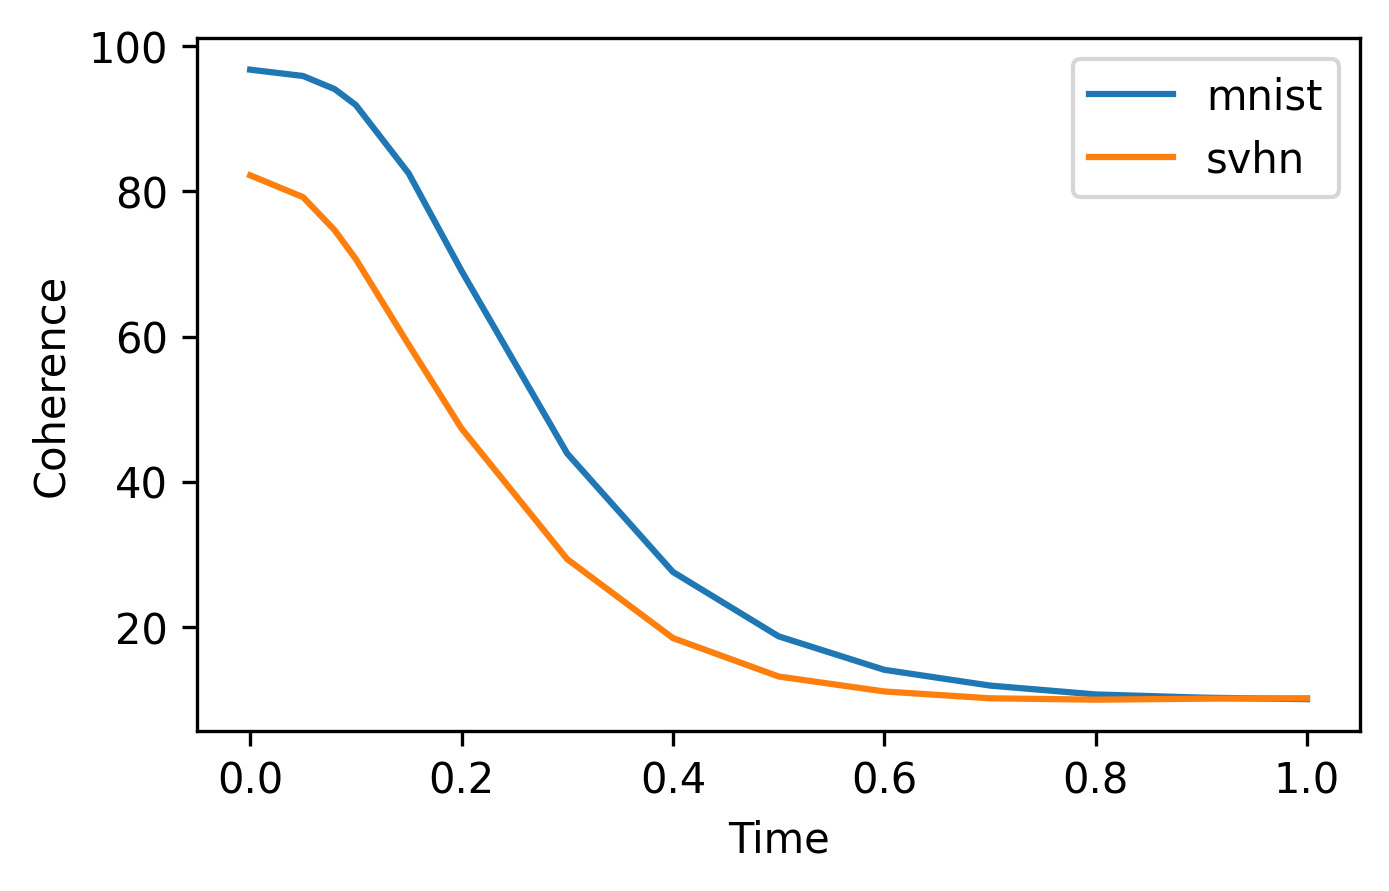
\includegraphics[page=1,width=\linewidth]{figures/plots/ms_latent_robustness}
         \caption{\mnist-\svhn}
     \end{subfigure}
        \begin{subfigure}[b]{0.3\textwidth}
         \centering
         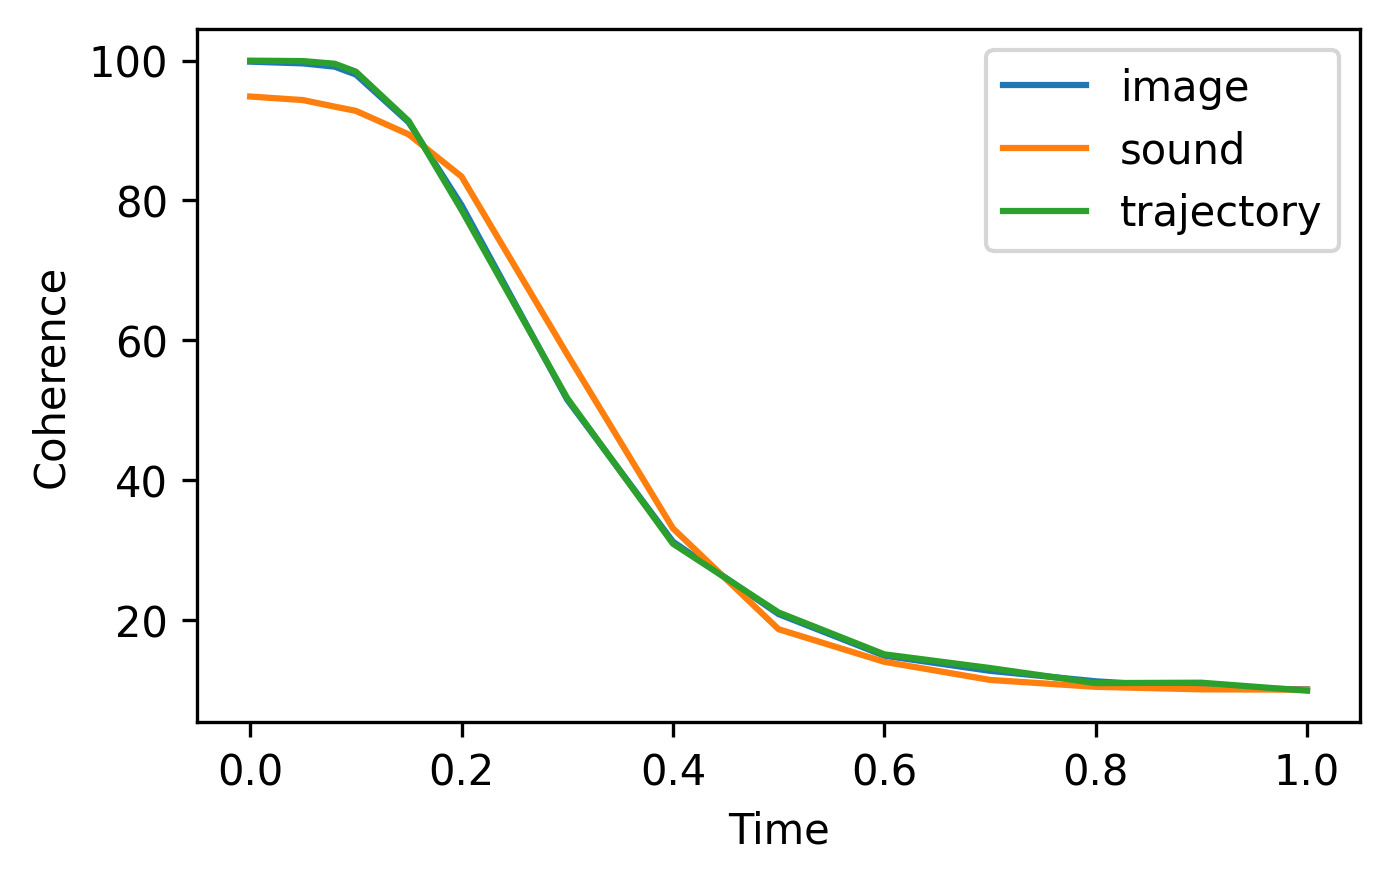
\includegraphics[page=1,width=\linewidth]{figures/plots/mhd_latent_robustness}
          \caption{\mhd}
     \end{subfigure}
      \begin{subfigure}[b]{0.3\textwidth}
         \centering
         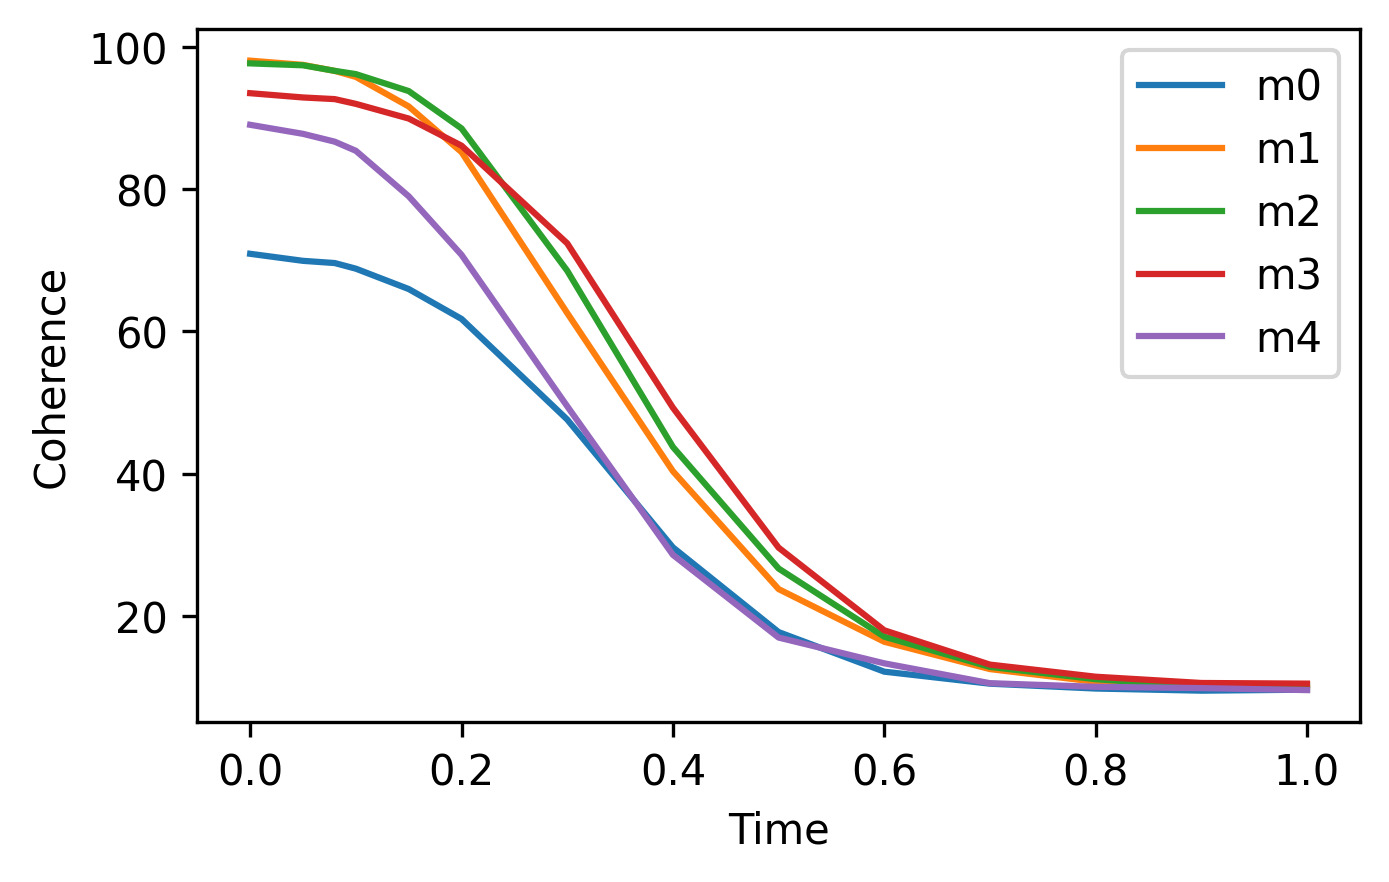
\includegraphics[page=1,width=\linewidth]{figures/plots/mmnist_latent_robustness}
            \caption{\polymnist}
     \end{subfigure}
   
        \caption{The coherence as a function of the diffusion process time for three datasets.  The diffusion perturbation is applied on the modalities latent space after an element wise normalization.}
        \label{fig:robust_exp}
\end{figure}






\subsection{Multi-time Masked Multi-modal SDE}

To learn the score network capable of both conditional and joint generation, we proposed in \Cref{sec:mld_var} a multi-time masked diffusion process. 

\Cref{algo:MLD_training} presents a pseudo-code for the multi time masked training. The masked diffusion process is applied following a randomization with probably $d$. First, a subset of modalities $A_2$ is selected randomly to be the conditioning modalities and $A_1$ the remaining set of modalities to be the diffused modalities. The time $t$ is sampled uniformly from $[0,T]$ and the portion of the latent space corresponding to the subset $A_1$ is diffused accordingly. Using the masking as shown in \Cref{train_line_mask}, the portion of the latent space corresponding to the subset $A_2$ is not diffused and forced to be equal to $R_0^{A_2} = z^{A_2}$. The multi-time vector $\tau$ is constructed. Lastly, the score network is optimized by minimizing a masked loss corresponding to the diffused part of the latent space. With probability $(1- d)$, all the modalities are diffused at the same time and $A_2 =\emptyset$. In order to calibrate the loss, given that the randomization of $A_1$ and $A_2$ can result in diffusing different sizes of the latent space, we re-weight the loss according to the cardinality of the diffused and freezed portions of the latent space:

\begin{equation} \label{eq:weight_eq}
    \Omega(A_1,A_2) = 1 + \frac{dim(A_2)}{dim(A_1)}
\end{equation}
Where $\dim(.) $ is the sum of each latent space cardinality of a given subset of modalities with $dim(\emptyset) = 0 $ .





\begin{algorithm}[hbt!]
\DontPrintSemicolon
\SetAlgoLined
\SetNoFillComment
\LinesNotNumbered 
\caption{\gls{MLD} Masked Multi-time diffusion training step}\label{algo:MLD_training}
\KwData{$ X = \{x^i\}_{i=1}^M $}
\textbf{Param:} $d$ \\
$Z \gets \{ e_{\phi_i}(x^i) \}_{i=0}^M $   \tcp*{Encode the modalities $X$ into their latent space } 
 $A_2 \sim \nu  \quad $ \tcp*{$\nu$ depends on the parameter $d$}
$A_1\gets \{1,\dots,M\}\setminus A_2 $ \\
$t \sim \mathcal{U}[0,T]$ \\

$R  \sim  q (r|Z,t) $ \tcp*{Diffuse the available portion of the latent space(\Cref{eq:diffuson_kernel})}
$R \gets m(A_1) \odot R     + (1- m(A_1) ) \odot Z$ \tcp*{Masked diffusion}  \label{train_line_mask}
$\tau(A_1,t) \gets \left[\mathds{1}(1\in A_1)t,\dots,\mathds{1}(M\in A_1)t\right]$ \tcp*{Construct the multi time vector} 

\textbf{Return} $ \nabla_{\chi} \left\{  \Omega(A_1,A_2) \quad  \norm{m(A_1)\odot \quad \left [  s_{\chi}(R,\tau(A_1,t))-\nabla \log q(R,t|z^{A_2})  \right]     }^2_2   \quad \right\} $

\end{algorithm}

The optimized score network can approximate both the conditional and unconditional true score:
\begin{equation}
    s_\chi(R_t,\tau(A_1,t)) \sim  \nabla\log q(R_t,t\g z^{A_2})).
\end{equation}
The joint generation is a special case of the latter with $A_2 = \emptyset$:
\begin{equation}
    s_\chi(R_t,\tau(A_1,t)) \sim  \nabla\log q(R_t,t) \quad     ,A_1 = \{1,...,M\}
\end{equation}

\Cref{algo:MLD_cond_gen} describes the reverse conditional generation pseudo-code. It's pertinent to compare this algorithm with \Cref{algo:MLD_inpaint_cond}. The main difference resides in the use of the multi-time score network, enabling conditional generation with the multi-time vector playing the role of time information and conditioning signal. On the other hand, in \Cref{algo:MLD_inpaint_cond}, we don't have a conditional score network, therefore we resort to the approximation from \Cref{sec:inpainting}, and use the unconditional score. 


\begin{algorithm}[hbt!]
\DontPrintSemicolon
\SetAlgoLined
\SetNoFillComment
\LinesNotNumbered 
\caption{MLD conditional generation.}\label{algo:MLD_cond_gen}
\KwData{$ x^{A_2} \gets \{ x^i\}_{i \in A_2} $ }  
$z^{A_2} \gets \{ e_{\phi_i}(x^i) \}_{i \in A_2} $   \tcp*{Encode the available modalities $X$ into their latent space} 
$A_1\gets \{1,\dots,M\}\setminus A_2 $ \tcp*{The set of modalities to be generated} 
$R_0 \gets \mathcal{C} ( R_0^{A_1}, z^{A_2}),  \qquad  R_0^{A_1} \sim \rho(r^{A_1}) $  \tcp*{Compose the initial latent space} 
$R \gets R_0$\\
$\Delta t \gets \nicefrac{T}{N}$ \\
\For{$n = 0  \quad \textbf{to} \quad N-1 \quad  $}{
$t' \gets T -  n  \ \Delta t $ \\
$\tau(A_1,t') \gets \left[\mathds{1}(1\in A_1)t',\dots,\mathds{1}(M\in A_1)t'\right]$ \tcp*{Construct the multi-time vector}
$\epsilon \sim \mathcal{N}(0;I)  \quad$  \textbf{if} $ n < N \quad  $ \textbf{else} $ \quad\epsilon= 0$ \\
$\Delta R  \gets  \Delta t \left[ \frac{1}{2} \beta(t') R  + \beta(t') s_\chi (R, \tau(A_1,t')) \right]  + \sqrt{\beta(t') \Delta t }  \epsilon   $ \\
$R \gets R +  \Delta R $ \tcp*{The Euler-Maruyama update step }
$R \gets m(A_1) \odot R + (1 -  m(A_1) )\odot R_{0} $  \tcp*{ Update the portion corresponding to the unavailable modalities }
} 
$ \hat{z}^{A_1} = R^{A_1}$ \\
\textbf{Return} $\hat{X}^{A_1} = \{d^i_\theta(\hat{z}^{i} )\}_{i\in A_1}$  
\end{algorithm}

\subsection{Uni-diffuser Training}
The work presented in \cite{bao2023transformer} is specialized for an image-caption application. The approach is based on a multi-modal diffusion model applied to a unified latent embedding, obtained via pre-trained autoencoders, and incorporating pre-trained models (CLIP \cite{radford2021clip} and GPT-2 \cite{radford2019language}). The unified latent space is composed of an image embedding, a CLIP image embedding and a CLIP text embedding. Note that the CLIP model is pre-trained on a pairs of multi-modal data (image-text), which is expected to enhance the generative performance. Since it is not trivial to have a jointly trained encoder similar to CLIP for any type of modality, the evaluation of this model on different modalities across different data-set (e.g. including audio) is not an easy task.

To compare to this work, we adapt the training scheme presented in \cite{bao2023transformer} to our \gls{MLD} method. Instead of applying a masked multi-modal \gls{SDE} for training the score network, every portion of the latent space is diffused according to a different time $t^i \sim \mathcal{U}(0,1)$ and, therefore, the multi-time vector fed to the score network is $\tau(t) = [t^0 \sim \mathcal{U}(0,1),..., t^M \sim \mathcal{U}(0,1) ] $. For fairness, we use the same score network and reverse process sampler as for our \gls{MLD} version with multi-time training, and call this variant \gls{MLD Uni}.

% {\color{blue}
\subsection{Intuitive summary: How does MLD capture modality interactions?}



\gls{MLD} treats the latent spaces of each modality as variables that evolve differently through the diffusion process according to a multi-time vector. %The joint score is learned by diffusing all the modalities at the same diffusion time whereas .
The masked multi-time training enables the model to learn the score of all the combination of conditionally diffused modalities, using the frozen modalities as the conditioning signal, through a randomized scheme. By learning the score function of the diffused modalities at different time steps, the score model captures the correlation between the modalities. At test time, the diffusion time of each modality is chosen to modulate its influence on the generation, as follows. 

For joint generation the model uses the unconditional score which corresponds to using the same diffusion time for all modalities. Thus, all the modalities influence each other equally. This ensures that modality interaction information is faithful to the one characterizing the observed data distribution. 

The model can also generate modalities conditionally by using the conditional score, by freezing the conditioning modalities during the reverse process. The freezed state is similar to the final state of the revere process where information is not perturbed, thus the influence of the conditioning modalities is maximal. Subsequently, the generated modalities reflect the necessary information from the conditioning modalities and achieve the desired correlation.
% }


\subsection{Technical details}

\paragraph{Sampling schedule:}
\label{sec:repaint_sche}
We use the sampling schedule proposed in \cite{lugmayr2022repaint}, which has shown to improve the coherence of the conditional and joint generation. We use the best parameters suggested by the authors: $N = 250$ time-steps, applied $r = 10$ re-sampling times with jump size $j = 10$. For readability in \cref{algo:MLD_inpaint_cond} and \cref{algo:MLD_cond_gen},  we present pseudo code  with a linear sampling schedule which can be easily adapted to any other schedule.

\paragraph{Training the score network: }
Inspired by the architecture from \citep{dupont22_fucnta}, we use simple Residual \gls{MLP} blocks with skip connections as our score network (see \Cref{fig:score_net}). We fix the \textbf{width} and \textbf{number of blocks} proportionally to the number of the modalities and the latent space size. As in \cite{song2020improved}, we use \gls{EMA} of model parameters with a momentum parameter $m = 0.999$.



\begin{figure}[h]
\centering


\tikzset{every picture/.style={line width=0.75pt}} %set default line width to 0.75pt        

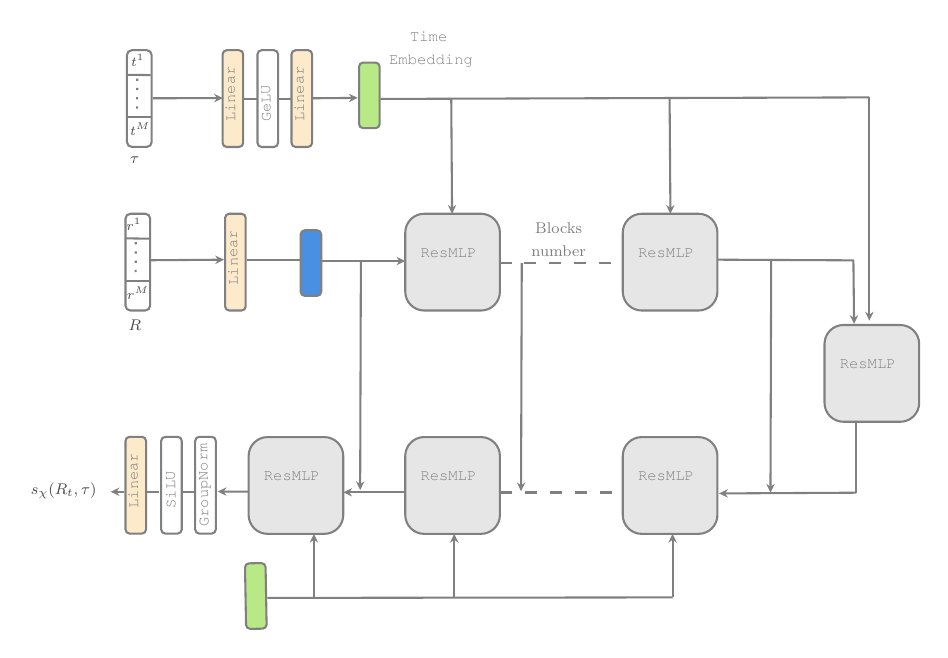
\begin{tikzpicture}[x=0.75pt,y=0.75pt,yscale=-1,xscale=1,scale=0.8]
%uncomment if require: \path (0,445); %set diagram left start at 0, and has height of 445

%Rounded Rect [id:dp45116577877352726] 
\draw  [color={rgb, 255:red, 128; green, 128; blue, 128 }  ,draw opacity=1 ][fill={rgb, 255:red, 245; green, 166; blue, 35 }  ,fill opacity=0.24 ] (121.6,35.48) .. controls (121.6,34.11) and (122.71,33) .. (124.08,33) -- (131.52,33) .. controls (132.89,33) and (134,34.11) .. (134,35.48) -- (134,88.8) .. controls (134,90.17) and (132.89,91.28) .. (131.52,91.28) -- (124.08,91.28) .. controls (122.71,91.28) and (121.6,90.17) .. (121.6,88.8) -- cycle ;

%Rounded Rect [id:dp6629173804221007] 
\draw  [color={rgb, 255:red, 128; green, 128; blue, 128 }  ,draw opacity=1 ][fill={rgb, 255:red, 255; green, 255; blue, 255 }  ,fill opacity=1 ] (142.6,35.48) .. controls (142.6,34.11) and (143.71,33) .. (145.08,33) -- (152.52,33) .. controls (153.89,33) and (155,34.11) .. (155,35.48) -- (155,88.8) .. controls (155,90.17) and (153.89,91.28) .. (152.52,91.28) -- (145.08,91.28) .. controls (143.71,91.28) and (142.6,90.17) .. (142.6,88.8) -- cycle ;

%Rounded Rect [id:dp23369966317189172] 
\draw  [color={rgb, 255:red, 128; green, 128; blue, 128 }  ,draw opacity=1 ][fill={rgb, 255:red, 245; green, 166; blue, 35 }  ,fill opacity=0.24 ] (163.1,35.48) .. controls (163.1,34.11) and (164.21,33) .. (165.58,33) -- (173.02,33) .. controls (174.39,33) and (175.5,34.11) .. (175.5,35.48) -- (175.5,88.8) .. controls (175.5,90.17) and (174.39,91.28) .. (173.02,91.28) -- (165.58,91.28) .. controls (164.21,91.28) and (163.1,90.17) .. (163.1,88.8) -- cycle ;

%Rounded Rect [id:dp47916639498650393] 
\draw  [color={rgb, 255:red, 128; green, 128; blue, 128 }  ,draw opacity=1 ][fill={rgb, 255:red, 184; green, 233; blue, 134 }  ,fill opacity=1 ] (203.77,42.93) .. controls (203.77,41.56) and (204.88,40.45) .. (206.25,40.45) -- (213.69,40.45) .. controls (215.06,40.45) and (216.17,41.56) .. (216.17,42.93) -- (216.17,77.47) .. controls (216.17,78.84) and (215.06,79.95) .. (213.69,79.95) -- (206.25,79.95) .. controls (204.88,79.95) and (203.77,78.84) .. (203.77,77.47) -- cycle ;
%Rounded Rect [id:dp16876487903558512] 
\draw  [color={rgb, 255:red, 128; green, 128; blue, 128 }  ,draw opacity=1 ][fill={rgb, 255:red, 245; green, 166; blue, 35 }  ,fill opacity=0.24 ] (123.1,133.98) .. controls (123.1,132.61) and (124.21,131.5) .. (125.58,131.5) -- (133.02,131.5) .. controls (134.39,131.5) and (135.5,132.61) .. (135.5,133.98) -- (135.5,187.3) .. controls (135.5,188.67) and (134.39,189.78) .. (133.02,189.78) -- (125.58,189.78) .. controls (124.21,189.78) and (123.1,188.67) .. (123.1,187.3) -- cycle ;

%Rounded Rect [id:dp8420620309987483] 
\draw  [color={rgb, 255:red, 128; green, 128; blue, 128 }  ,draw opacity=1 ][fill={rgb, 255:red, 74; green, 144; blue, 226 }  ,fill opacity=1 ] (168.6,143.93) .. controls (168.6,142.56) and (169.71,141.45) .. (171.08,141.45) -- (178.52,141.45) .. controls (179.89,141.45) and (181,142.56) .. (181,143.93) -- (181,178.47) .. controls (181,179.84) and (179.89,180.95) .. (178.52,180.95) -- (171.08,180.95) .. controls (169.71,180.95) and (168.6,179.84) .. (168.6,178.47) -- cycle ;
%Rounded Rect [id:dp43011173971404815] 
\draw  [color={rgb, 255:red, 128; green, 128; blue, 128 }  ,draw opacity=1 ][fill={rgb, 255:red, 245; green, 166; blue, 35 }  ,fill opacity=0.24 ] (63.1,268.31) .. controls (63.1,266.94) and (64.21,265.83) .. (65.58,265.83) -- (73.02,265.83) .. controls (74.39,265.83) and (75.5,266.94) .. (75.5,268.31) -- (75.5,321.63) .. controls (75.5,323) and (74.39,324.11) .. (73.02,324.11) -- (65.58,324.11) .. controls (64.21,324.11) and (63.1,323) .. (63.1,321.63) -- cycle ;

%Rounded Rect [id:dp7382623771259675] 
\draw  [color={rgb, 255:red, 128; green, 128; blue, 128 }  ,draw opacity=1 ][fill={rgb, 255:red, 255; green, 255; blue, 255 }  ,fill opacity=1 ] (105.1,268.31) .. controls (105.1,266.94) and (106.21,265.83) .. (107.58,265.83) -- (115.02,265.83) .. controls (116.39,265.83) and (117.5,266.94) .. (117.5,268.31) -- (117.5,321.63) .. controls (117.5,323) and (116.39,324.11) .. (115.02,324.11) -- (107.58,324.11) .. controls (106.21,324.11) and (105.1,323) .. (105.1,321.63) -- cycle ;
%Rounded Rect [id:dp740256948923222] 
\draw  [color={rgb, 255:red, 128; green, 128; blue, 128 }  ,draw opacity=1 ][fill={rgb, 255:red, 255; green, 255; blue, 255 }  ,fill opacity=1 ] (84.6,268.31) .. controls (84.6,266.94) and (85.71,265.83) .. (87.08,265.83) -- (94.52,265.83) .. controls (95.89,265.83) and (97,266.94) .. (97,268.31) -- (97,321.63) .. controls (97,323) and (95.89,324.11) .. (94.52,324.11) -- (87.08,324.11) .. controls (85.71,324.11) and (84.6,323) .. (84.6,321.63) -- cycle ;
%Rounded Rect [id:dp18399833106662933] 
\draw  [color={rgb, 255:red, 128; green, 128; blue, 128 }  ,draw opacity=1 ][fill={rgb, 255:red, 128; green, 128; blue, 128 }  ,fill opacity=0.2 ] (362.6,142.9) .. controls (362.6,136.6) and (367.7,131.5) .. (374,131.5) -- (408.2,131.5) .. controls (414.5,131.5) and (419.6,136.6) .. (419.6,142.9) -- (419.6,178.38) .. controls (419.6,184.68) and (414.5,189.78) .. (408.2,189.78) -- (374,189.78) .. controls (367.7,189.78) and (362.6,184.68) .. (362.6,178.38) -- cycle ;

%Rounded Rect [id:dp6859408399476166] 
\draw  [color={rgb, 255:red, 128; green, 128; blue, 128 }  ,draw opacity=1 ][fill={rgb, 255:red, 128; green, 128; blue, 128 }  ,fill opacity=0.2 ] (484.1,209.9) .. controls (484.1,203.6) and (489.2,198.5) .. (495.5,198.5) -- (529.7,198.5) .. controls (536,198.5) and (541.1,203.6) .. (541.1,209.9) -- (541.1,245.38) .. controls (541.1,251.68) and (536,256.78) .. (529.7,256.78) -- (495.5,256.78) .. controls (489.2,256.78) and (484.1,251.68) .. (484.1,245.38) -- cycle ;

%Rounded Rect [id:dp842740857754539] 
\draw  [color={rgb, 255:red, 128; green, 128; blue, 128 }  ,draw opacity=1 ][fill={rgb, 255:red, 128; green, 128; blue, 128 }  ,fill opacity=0.2 ] (362.6,277.4) .. controls (362.6,271.1) and (367.7,266) .. (374,266) -- (408.2,266) .. controls (414.5,266) and (419.6,271.1) .. (419.6,277.4) -- (419.6,312.88) .. controls (419.6,319.18) and (414.5,324.28) .. (408.2,324.28) -- (374,324.28) .. controls (367.7,324.28) and (362.6,319.18) .. (362.6,312.88) -- cycle ;

%Rounded Rect [id:dp10628875234333468] 
\draw  [color={rgb, 255:red, 128; green, 128; blue, 128 }  ,draw opacity=1 ][fill={rgb, 255:red, 128; green, 128; blue, 128 }  ,fill opacity=0.2 ] (231.6,277.4) .. controls (231.6,271.1) and (236.7,266) .. (243,266) -- (277.2,266) .. controls (283.5,266) and (288.6,271.1) .. (288.6,277.4) -- (288.6,312.88) .. controls (288.6,319.18) and (283.5,324.28) .. (277.2,324.28) -- (243,324.28) .. controls (236.7,324.28) and (231.6,319.18) .. (231.6,312.88) -- cycle ;

%Straight Lines [id:da15987670699550205] 
\draw [color={rgb, 255:red, 128; green, 128; blue, 128 }  ,draw opacity=1 ]   (511.1,61.42) -- (511.1,192.85) ;
\draw [shift={(511.1,195.85)}, rotate = 270] [fill={rgb, 255:red, 128; green, 128; blue, 128 }  ,fill opacity=1 ][line width=0.08]  [draw opacity=0] (5.36,-2.57) -- (0,0) -- (5.36,2.57) -- (3.56,0) -- cycle    ;
%Straight Lines [id:da39303184575868344] 
\draw [color={rgb, 255:red, 128; green, 128; blue, 128 }  ,draw opacity=1 ]   (216.6,62.35) -- (511.1,61.42) ;
%Straight Lines [id:da800059204600343] 
\draw [color={rgb, 255:red, 128; green, 128; blue, 128 }  ,draw opacity=1 ]   (390.8,61.95) -- (391.28,128.5) ;
\draw [shift={(391.3,131.5)}, rotate = 269.59] [fill={rgb, 255:red, 128; green, 128; blue, 128 }  ,fill opacity=1 ][line width=0.08]  [draw opacity=0] (5.36,-2.57) -- (0,0) -- (5.36,2.57) -- (3.56,0) -- cycle    ;
%Straight Lines [id:da7453494852796207] 
\draw [color={rgb, 255:red, 128; green, 128; blue, 128 }  ,draw opacity=1 ]   (259.3,61.95) -- (259.78,128.5) ;
\draw [shift={(259.8,131.5)}, rotate = 269.59] [fill={rgb, 255:red, 128; green, 128; blue, 128 }  ,fill opacity=1 ][line width=0.08]  [draw opacity=0] (5.36,-2.57) -- (0,0) -- (5.36,2.57) -- (3.56,0) -- cycle    ;
%Straight Lines [id:da2495969210189002] 
\draw [color={rgb, 255:red, 128; green, 128; blue, 128 }  ,draw opacity=1 ] [dash pattern={on 4.5pt off 4.5pt}]  (288.09,160.95) -- (362.09,160.95) ;
%Straight Lines [id:da8597197154488614] 
\draw [color={rgb, 255:red, 128; green, 128; blue, 128 }  ,draw opacity=1 ]   (181.12,159.96) -- (228.6,159.96) ;
\draw [shift={(231.6,159.96)}, rotate = 180] [fill={rgb, 255:red, 128; green, 128; blue, 128 }  ,fill opacity=1 ][line width=0.08]  [draw opacity=0] (5.36,-2.57) -- (0,0) -- (5.36,2.57) -- (3.56,0) -- cycle    ;
%Straight Lines [id:da33226462684386915] 
\draw [color={rgb, 255:red, 128; green, 128; blue, 128 }  ,draw opacity=1 ]   (419.6,159.16) -- (501.72,159.56) ;
%Straight Lines [id:da43782889035407124] 
\draw [color={rgb, 255:red, 128; green, 128; blue, 128 }  ,draw opacity=1 ]   (501.5,159.45) -- (501.87,194.85) ;
\draw [shift={(501.9,197.85)}, rotate = 269.4] [fill={rgb, 255:red, 128; green, 128; blue, 128 }  ,fill opacity=1 ][line width=0.08]  [draw opacity=0] (5.36,-2.57) -- (0,0) -- (5.36,2.57) -- (3.56,0) -- cycle    ;
%Straight Lines [id:da23578754948847647] 
\draw [color={rgb, 255:red, 128; green, 128; blue, 128 }  ,draw opacity=1 ]   (503.18,256.6) -- (503.18,299.49) ;
%Straight Lines [id:da8816929648715184] 
\draw [color={rgb, 255:red, 128; green, 128; blue, 128 }  ,draw opacity=1 ]   (423.6,299.92) -- (503.18,299.49) ;
\draw [shift={(420.6,299.93)}, rotate = 359.69] [fill={rgb, 255:red, 128; green, 128; blue, 128 }  ,fill opacity=1 ][line width=0.08]  [draw opacity=0] (5.36,-2.57) -- (0,0) -- (5.36,2.57) -- (3.56,0) -- cycle    ;
%Straight Lines [id:da11493937440242985] 
\draw [color={rgb, 255:red, 128; green, 128; blue, 128 }  ,draw opacity=1 ] [dash pattern={on 4.5pt off 4.5pt}]  (288.64,299.39) -- (362.64,299.39) ;
%Straight Lines [id:da869681082719342] 
\draw [color={rgb, 255:red, 128; green, 128; blue, 128 }  ,draw opacity=1 ]   (197.31,299.27) -- (231.6,299.27) ;
\draw [shift={(194.31,299.27)}, rotate = 0] [fill={rgb, 255:red, 128; green, 128; blue, 128 }  ,fill opacity=1 ][line width=0.08]  [draw opacity=0] (5.36,-2.57) -- (0,0) -- (5.36,2.57) -- (3.56,0) -- cycle    ;
%Straight Lines [id:da44612596689312034] 
\draw [color={rgb, 255:red, 128; green, 128; blue, 128 }  ,draw opacity=1 ]   (121.64,298.82) -- (136.8,298.83) ;
\draw [shift={(118.64,298.82)}, rotate = 0.04] [fill={rgb, 255:red, 128; green, 128; blue, 128 }  ,fill opacity=1 ][line width=0.08]  [draw opacity=0] (5.36,-2.57) -- (0,0) -- (5.36,2.57) -- (3.56,0) -- cycle    ;
%Straight Lines [id:da49219482761766953] 
\draw [color={rgb, 255:red, 128; green, 128; blue, 128 }  ,draw opacity=1 ]   (96.64,299.16) -- (104.87,299.16) ;
%Straight Lines [id:da744069622158885] 
\draw [color={rgb, 255:red, 128; green, 128; blue, 128 }  ,draw opacity=1 ]   (75.31,299.16) -- (83.53,299.16) ;
%Straight Lines [id:da013270848272890934] 
\draw [color={rgb, 255:red, 128; green, 128; blue, 128 }  ,draw opacity=1 ]   (57.2,298.93) -- (62.42,298.93) ;
\draw [shift={(54.2,298.93)}, rotate = 0] [fill={rgb, 255:red, 128; green, 128; blue, 128 }  ,fill opacity=1 ][line width=0.08]  [draw opacity=0] (5.36,-2.57) -- (0,0) -- (5.36,2.57) -- (3.56,0) -- cycle    ;
%Straight Lines [id:da29792639183075575] 
\draw [color={rgb, 255:red, 128; green, 128; blue, 128 }  ,draw opacity=1 ]   (136.09,159.49) -- (168.76,159.49) ;
%Straight Lines [id:da702427757163758] 
\draw [color={rgb, 255:red, 128; green, 128; blue, 128 }  ,draw opacity=1 ]   (134.64,62.13) -- (142.87,62.13) ;
%Straight Lines [id:da46605945347545785] 
\draw [color={rgb, 255:red, 128; green, 128; blue, 128 }  ,draw opacity=1 ]   (154.87,62.13) -- (163.09,62.13) ;
%Straight Lines [id:da6300259185680861] 
\draw [color={rgb, 255:red, 128; green, 128; blue, 128 }  ,draw opacity=1 ]   (175.56,61.96) -- (199.98,61.74) ;
\draw [shift={(202.98,61.71)}, rotate = 179.48] [fill={rgb, 255:red, 128; green, 128; blue, 128 }  ,fill opacity=1 ][line width=0.08]  [draw opacity=0] (5.36,-2.57) -- (0,0) -- (5.36,2.57) -- (3.56,0) -- cycle    ;
%Straight Lines [id:da8724877452780204] 
\draw [color={rgb, 255:red, 128; green, 128; blue, 128 }  ,draw opacity=1 ]   (451.99,159.2) -- (451.56,296.49) ;
\draw [shift={(451.56,299.49)}, rotate = 270.18] [fill={rgb, 255:red, 128; green, 128; blue, 128 }  ,fill opacity=1 ][line width=0.08]  [draw opacity=0] (5.36,-2.57) -- (0,0) -- (5.36,2.57) -- (3.56,0) -- cycle    ;
%Straight Lines [id:da5976028186816709] 
\draw [color={rgb, 255:red, 128; green, 128; blue, 128 }  ,draw opacity=1 ]   (301.77,161.18) -- (301.34,295.6) ;
\draw [shift={(301.33,298.6)}, rotate = 270.18] [fill={rgb, 255:red, 128; green, 128; blue, 128 }  ,fill opacity=1 ][line width=0.08]  [draw opacity=0] (5.36,-2.57) -- (0,0) -- (5.36,2.57) -- (3.56,0) -- cycle    ;
%Straight Lines [id:da1735182413440839] 
\draw [color={rgb, 255:red, 128; green, 128; blue, 128 }  ,draw opacity=1 ]   (204.88,160.49) -- (204.45,294.91) ;
\draw [shift={(204.44,297.91)}, rotate = 270.18] [fill={rgb, 255:red, 128; green, 128; blue, 128 }  ,fill opacity=1 ][line width=0.08]  [draw opacity=0] (5.36,-2.57) -- (0,0) -- (5.36,2.57) -- (3.56,0) -- cycle    ;
%Rounded Rect [id:dp5435791719991034] 
\draw  [color={rgb, 255:red, 128; green, 128; blue, 128 }  ,draw opacity=1 ][fill={rgb, 255:red, 184; green, 233; blue, 134 }  ,fill opacity=1 ] (148.1,378.86) .. controls (148.13,380.23) and (147.04,381.36) .. (145.67,381.38) -- (138.23,381.51) .. controls (136.86,381.54) and (135.73,380.45) .. (135.71,379.08) -- (135.1,344.54) .. controls (135.07,343.17) and (136.16,342.04) .. (137.53,342.02) -- (144.97,341.89) .. controls (146.34,341.86) and (147.47,342.95) .. (147.49,344.32) -- cycle ;
%Straight Lines [id:da5683776914233258] 
\draw [color={rgb, 255:red, 128; green, 128; blue, 128 }  ,draw opacity=1 ]   (148.6,362.85) -- (392.6,362.55) ;
%Straight Lines [id:da23839955840628768] 
\draw [color={rgb, 255:red, 128; green, 128; blue, 128 }  ,draw opacity=1 ]   (392.6,362.55) -- (392.6,327.28) ;
\draw [shift={(392.6,324.28)}, rotate = 90] [fill={rgb, 255:red, 128; green, 128; blue, 128 }  ,fill opacity=1 ][line width=0.08]  [draw opacity=0] (5.36,-2.57) -- (0,0) -- (5.36,2.57) -- (3.56,0) -- cycle    ;
%Straight Lines [id:da0923923318962463] 
\draw [color={rgb, 255:red, 128; green, 128; blue, 128 }  ,draw opacity=1 ]   (261.1,362.55) -- (261.1,327.28) ;
\draw [shift={(261.1,324.28)}, rotate = 90] [fill={rgb, 255:red, 128; green, 128; blue, 128 }  ,fill opacity=1 ][line width=0.08]  [draw opacity=0] (5.36,-2.57) -- (0,0) -- (5.36,2.57) -- (3.56,0) -- cycle    ;
%Straight Lines [id:da7721018720253876] 
\draw [color={rgb, 255:red, 128; green, 128; blue, 128 }  ,draw opacity=1 ]   (176.6,362.55) -- (176.6,327.28) ;
\draw [shift={(176.6,324.28)}, rotate = 90] [fill={rgb, 255:red, 128; green, 128; blue, 128 }  ,fill opacity=1 ][line width=0.08]  [draw opacity=0] (5.36,-2.57) -- (0,0) -- (5.36,2.57) -- (3.56,0) -- cycle    ;
%Rounded Rect [id:dp1551004112129395] 
\draw  [color={rgb, 255:red, 128; green, 128; blue, 128 }  ,draw opacity=1 ] (63.1,134.48) .. controls (63.1,132.83) and (64.43,131.5) .. (66.08,131.5) -- (75.02,131.5) .. controls (76.67,131.5) and (78,132.83) .. (78,134.48) -- (78,186.8) .. controls (78,188.45) and (76.67,189.78) .. (75.02,189.78) -- (66.08,189.78) .. controls (64.43,189.78) and (63.1,188.45) .. (63.1,186.8) -- cycle ;
%Straight Lines [id:da22891046032842355] 
\draw [color={rgb, 255:red, 128; green, 128; blue, 128 }  ,draw opacity=1 ]   (62.69,146.31) -- (77.33,146.51) ;
%Straight Lines [id:da8202528285215891] 
\draw [color={rgb, 255:red, 128; green, 128; blue, 128 }  ,draw opacity=1 ]   (62.97,171.74) -- (77.54,171.74) ;
%Straight Lines [id:da8432743896900226] 
\draw [color={rgb, 255:red, 128; green, 128; blue, 128 }  ,draw opacity=1 ] [dash pattern={on 0.84pt off 2.51pt}]  (69.31,148.57) -- (69.26,168.6) ;
%Rounded Rect [id:dp9973810427181078] 
\draw  [color={rgb, 255:red, 128; green, 128; blue, 128 }  ,draw opacity=1 ] (63.99,35.97) .. controls (63.99,34.32) and (65.32,32.99) .. (66.97,32.99) -- (75.91,32.99) .. controls (77.55,32.99) and (78.89,34.32) .. (78.89,35.97) -- (78.89,88.29) .. controls (78.89,89.93) and (77.55,91.27) .. (75.91,91.27) -- (66.97,91.27) .. controls (65.32,91.27) and (63.99,89.93) .. (63.99,88.29) -- cycle ;
%Straight Lines [id:da5612285806326431] 
\draw [color={rgb, 255:red, 128; green, 128; blue, 128 }  ,draw opacity=1 ]   (63.57,47.8) -- (78.22,48) ;
%Straight Lines [id:da22094837222694874] 
\draw [color={rgb, 255:red, 128; green, 128; blue, 128 }  ,draw opacity=1 ]   (63.86,73.23) -- (78.43,73.23) ;
%Straight Lines [id:da9238260217302401] 
\draw [color={rgb, 255:red, 128; green, 128; blue, 128 }  ,draw opacity=1 ] [dash pattern={on 0.84pt off 2.51pt}]  (70.2,50.06) -- (70.15,70.09) ;
%Straight Lines [id:da9054213973773921] 
\draw [color={rgb, 255:red, 128; green, 128; blue, 128 }  ,draw opacity=1 ]   (79.56,61.96) -- (118.8,61.84) ;
\draw [shift={(121.8,61.83)}, rotate = 179.83] [fill={rgb, 255:red, 128; green, 128; blue, 128 }  ,fill opacity=1 ][line width=0.08]  [draw opacity=0] (5.36,-2.57) -- (0,0) -- (5.36,2.57) -- (3.56,0) -- cycle    ;
%Straight Lines [id:da8899885040638749] 
\draw [color={rgb, 255:red, 128; green, 128; blue, 128 }  ,draw opacity=1 ]   (78.47,159.5) -- (119.47,159.19) ;
\draw [shift={(122.47,159.17)}, rotate = 179.57] [fill={rgb, 255:red, 128; green, 128; blue, 128 }  ,fill opacity=1 ][line width=0.08]  [draw opacity=0] (5.36,-2.57) -- (0,0) -- (5.36,2.57) -- (3.56,0) -- cycle    ;
%Rounded Rect [id:dp7103406473117098] 
\draw  [color={rgb, 255:red, 128; green, 128; blue, 128 }  ,draw opacity=1 ][fill={rgb, 255:red, 128; green, 128; blue, 128 }  ,fill opacity=0.2 ] (231.6,142.9) .. controls (231.6,136.6) and (236.7,131.5) .. (243,131.5) -- (277.2,131.5) .. controls (283.5,131.5) and (288.6,136.6) .. (288.6,142.9) -- (288.6,178.38) .. controls (288.6,184.68) and (283.5,189.78) .. (277.2,189.78) -- (243,189.78) .. controls (236.7,189.78) and (231.6,184.68) .. (231.6,178.38) -- cycle ;

%Rounded Rect [id:dp8954536542347509] 
\draw  [color={rgb, 255:red, 128; green, 128; blue, 128 }  ,draw opacity=1 ][fill={rgb, 255:red, 128; green, 128; blue, 128 }  ,fill opacity=0.2 ] (137.27,277.4) .. controls (137.27,271.1) and (142.37,266) .. (148.67,266) -- (182.87,266) .. controls (189.16,266) and (194.27,271.1) .. (194.27,277.4) -- (194.27,312.88) .. controls (194.27,319.18) and (189.16,324.28) .. (182.87,324.28) -- (148.67,324.28) .. controls (142.37,324.28) and (137.27,319.18) .. (137.27,312.88) -- cycle ;


% Text Node
\draw (121.86,77.64) node [anchor=north west][inner sep=0.75pt]  [font=\scriptsize,rotate=-269.05,xscale=0.7,yscale=0.7] [align=left] {{\fontfamily{pcr}\selectfont \textcolor[rgb]{0.5,0.5,0.5}{{\footnotesize Linear}}}};
% Text Node
\draw (163.36,77.64) node [anchor=north west][inner sep=0.75pt]  [font=\scriptsize,rotate=-269.05,xscale=0.7,yscale=0.7] [align=left] {{\fontfamily{pcr}\selectfont \textcolor[rgb]{0.5,0.5,0.5}{{\footnotesize Linear}}}};
% Text Node
\draw (123.36,176.14) node [anchor=north west][inner sep=0.75pt]  [font=\scriptsize,rotate=-269.05,xscale=0.7,yscale=0.7] [align=left] {{\fontfamily{pcr}\selectfont \textcolor[rgb]{0.5,0.5,0.5}{{\footnotesize Linear}}}};
% Text Node
\draw (63.36,310.47) node [anchor=north west][inner sep=0.75pt]  [font=\scriptsize,rotate=-269.05,xscale=0.7,yscale=0.7] [align=left] {{\fontfamily{pcr}\selectfont \textcolor[rgb]{0.5,0.5,0.5}{{\footnotesize Linear}}}};
% Text Node
\draw (143.86,77.64) node [anchor=north west][inner sep=0.75pt]  [font=\scriptsize,rotate=-269.05,xscale=0.7,yscale=0.7] [align=left] {{\fontfamily{pcr}\selectfont \textcolor[rgb]{0.5,0.5,0.5}{{\footnotesize GeLU}}}};
% Text Node
\draw (106.36,321.47) node [anchor=north west][inner sep=0.75pt]  [font=\tiny,rotate=-269.05,xscale=0.7,yscale=0.7] [align=left] {{\fontfamily{pcr}\selectfont \textcolor[rgb]{0.5,0.5,0.5}{{\footnotesize GroupNorm}}}};
% Text Node
\draw (370.5,151) node [anchor=north west][inner sep=0.75pt]  [xscale=0.7,yscale=0.7] [align=left] {{\footnotesize {\fontfamily{pcr}\selectfont \textcolor[rgb]{0.5,0.5,0.5}{ResMLP}}}};
% Text Node
\draw (492,218) node [anchor=north west][inner sep=0.75pt]  [xscale=0.7,yscale=0.7] [align=left] {{\footnotesize {\fontfamily{pcr}\selectfont \textcolor[rgb]{0.5,0.5,0.5}{ResMLP}}}};
% Text Node
\draw (370.5,285.5) node [anchor=north west][inner sep=0.75pt]  [xscale=0.7,yscale=0.7] [align=left] {{\footnotesize {\fontfamily{pcr}\selectfont \textcolor[rgb]{0.5,0.5,0.5}{ResMLP}}}};
% Text Node
\draw (239.5,285.5) node [anchor=north west][inner sep=0.75pt]  [xscale=0.7,yscale=0.7] [align=left] {{\footnotesize {\fontfamily{pcr}\selectfont \textcolor[rgb]{0.5,0.5,0.5}{ResMLP}}}};
% Text Node
\draw (303.6,135.5) node [anchor=north west][inner sep=0.75pt]  [xscale=0.7,yscale=0.7] [align=left] {\begin{minipage}[lt]{32.66pt}\setlength\topsep{0pt}
\begin{center}
\textcolor[rgb]{0.5,0.5,0.5}{{\footnotesize Blocks}}\\\textcolor[rgb]{0.5,0.5,0.5}{{\footnotesize  number}}
\end{center}

\end{minipage}};
% Text Node
\draw (220.6,20.06) node [anchor=north west][inner sep=0.75pt]  [xscale=0.7,yscale=0.7] [align=left] {\begin{minipage}[lt]{40.83pt}\setlength\topsep{0pt}
\begin{center}
\textcolor[rgb]{0.5,0.5,0.5}{{\footnotesize {\fontfamily{pcr}\selectfont Time}}}\\{\fontfamily{pcr}\selectfont \textcolor[rgb]{0.5,0.5,0.5}{{\footnotesize Embedding}}}
\end{center}

\end{minipage}};
% Text Node
\draw (63.64,194.18) node [anchor=north west][inner sep=0.75pt]  [font=\footnotesize,color={rgb, 255:red, 74; green, 74; blue, 74 }  ,opacity=1 ,xscale=0.7,yscale=0.7]  {$R$};
% Text Node
\draw (62.28,132.9) node [anchor=north west][inner sep=0.75pt]  [font=\scriptsize,color={rgb, 255:red, 74; green, 74; blue, 74 }  ,opacity=1 ,xscale=0.7,yscale=0.7]  {$r^{1}$};
% Text Node
\draw (62.71,174.18) node [anchor=north west][inner sep=0.75pt]  [font=\scriptsize,color={rgb, 255:red, 74; green, 74; blue, 74 }  ,opacity=1 ,xscale=0.7,yscale=0.7]  {$r^{M}$};
% Text Node
\draw (64.53,95.67) node [anchor=north west][inner sep=0.75pt]  [font=\footnotesize,color={rgb, 255:red, 74; green, 74; blue, 74 }  ,opacity=1 ,xscale=0.7,yscale=0.7]  {$\tau $};
% Text Node
\draw (65.17,34.39) node [anchor=north west][inner sep=0.75pt]  [font=\scriptsize,color={rgb, 255:red, 74; green, 74; blue, 74 }  ,opacity=1 ,xscale=0.7,yscale=0.7]  {$t^{1}$};
% Text Node
\draw (64.6,75.67) node [anchor=north west][inner sep=0.75pt]  [font=\scriptsize,color={rgb, 255:red, 74; green, 74; blue, 74 }  ,opacity=1 ,xscale=0.7,yscale=0.7]  {$t^{M}$};
% Text Node
\draw (4.83,292.23) node [anchor=north west][inner sep=0.75pt]  [font=\footnotesize,xscale=0.7,yscale=0.7]  {$\textcolor[rgb]{0.29,0.29,0.29}{s}\textcolor[rgb]{0.29,0.29,0.29}{_{\chi }}\textcolor[rgb]{0.29,0.29,0.29}{(}\textcolor[rgb]{0.29,0.29,0.29}{R_{t} ,\tau }\textcolor[rgb]{0.29,0.29,0.29}{)}$};
% Text Node
\draw (85.86,310.47) node [anchor=north west][inner sep=0.75pt]  [font=\scriptsize,rotate=-269.05,xscale=0.7,yscale=0.7] [align=left] {{\fontfamily{pcr}\selectfont \textcolor[rgb]{0.5,0.5,0.5}{{\footnotesize SiLU}}}};
% Text Node
\draw (239.5,151) node [anchor=north west][inner sep=0.75pt]  [xscale=0.7,yscale=0.7] [align=left] {{\footnotesize {\fontfamily{pcr}\selectfont \textcolor[rgb]{0.5,0.5,0.5}{ResMLP}}}};
% Text Node
\draw (145.17,285.5) node [anchor=north west][inner sep=0.75pt]  [xscale=0.7,yscale=0.7] [align=left] {{\footnotesize {\fontfamily{pcr}\selectfont \textcolor[rgb]{0.5,0.5,0.5}{ResMLP}}}};


\end{tikzpicture}

\caption{Score network $s_\chi$ architecture used in our \gls{MLD} implementation. Residual \gls{MLP} block architecture is shown in \Cref{fig:resmlp}.}
\label{fig:score_net}
\end{figure}

\begin{figure}[h]
    \centering
    

\tikzset{every picture/.style={line width=0.75pt}} %set default line width to 0.75pt        

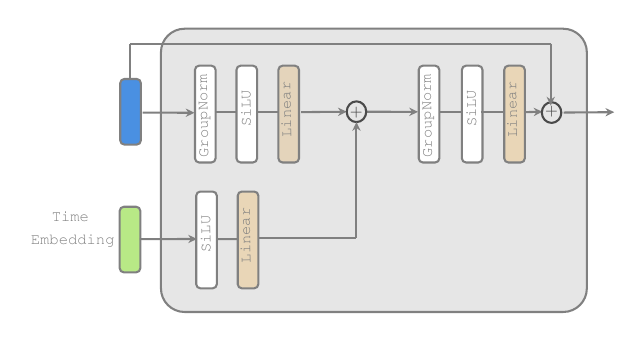
\begin{tikzpicture}[x=0.75pt,y=0.75pt,yscale=-1,xscale=1,scale=0.8]
%uncomment if require: \path (0,199); %set diagram left start at 0, and has height of 199

%Rounded Rect [id:dp23369966317189172] 
\draw  [color={rgb, 255:red, 128; green, 128; blue, 128 }  ,draw opacity=1 ][fill={rgb, 255:red, 245; green, 166; blue, 35 }  ,fill opacity=0.24 ] (361.85,35.48) .. controls (361.85,34.11) and (362.96,33) .. (364.33,33) -- (371.77,33) .. controls (373.14,33) and (374.25,34.11) .. (374.25,35.48) -- (374.25,88.8) .. controls (374.25,90.17) and (373.14,91.28) .. (371.77,91.28) -- (364.33,91.28) .. controls (362.96,91.28) and (361.85,90.17) .. (361.85,88.8) -- cycle ;

%Rounded Rect [id:dp47916639498650393] 
\draw  [color={rgb, 255:red, 128; green, 128; blue, 128 }  ,draw opacity=1 ][fill={rgb, 255:red, 184; green, 233; blue, 134 }  ,fill opacity=1 ] (266.27,120.43) .. controls (266.27,119.06) and (267.38,117.95) .. (268.75,117.95) -- (276.19,117.95) .. controls (277.56,117.95) and (278.67,119.06) .. (278.67,120.43) -- (278.67,154.97) .. controls (278.67,156.34) and (277.56,157.45) .. (276.19,157.45) -- (268.75,157.45) .. controls (267.38,157.45) and (266.27,156.34) .. (266.27,154.97) -- cycle ;
%Rounded Rect [id:dp8420620309987483] 
\draw  [color={rgb, 255:red, 128; green, 128; blue, 128 }  ,draw opacity=1 ][fill={rgb, 255:red, 74; green, 144; blue, 226 }  ,fill opacity=1 ] (266.6,43.48) .. controls (266.6,42.11) and (267.71,41) .. (269.08,41) -- (276.52,41) .. controls (277.89,41) and (279,42.11) .. (279,43.48) -- (279,78.02) .. controls (279,79.39) and (277.89,80.5) .. (276.52,80.5) -- (269.08,80.5) .. controls (267.71,80.5) and (266.6,79.39) .. (266.6,78.02) -- cycle ;
%Rounded Rect [id:dp4961571836770784] 
\draw  [color={rgb, 255:red, 128; green, 128; blue, 128 }  ,draw opacity=1 ][fill={rgb, 255:red, 128; green, 128; blue, 128 }  ,fill opacity=0.2 ] (291.1,24.97) .. controls (291.1,17.1) and (297.48,10.72) .. (305.35,10.72) -- (533.35,10.72) .. controls (541.22,10.72) and (547.6,17.1) .. (547.6,24.97) -- (547.6,167.07) .. controls (547.6,174.94) and (541.22,181.32) .. (533.35,181.32) -- (305.35,181.32) .. controls (297.48,181.32) and (291.1,174.94) .. (291.1,167.07) -- cycle ;
%Rounded Rect [id:dp43011173971404815] 
\draw  [color={rgb, 255:red, 128; green, 128; blue, 128 }  ,draw opacity=1 ][fill={rgb, 255:red, 245; green, 166; blue, 35 }  ,fill opacity=0.24 ] (337.35,111.27) .. controls (337.35,109.9) and (338.46,108.79) .. (339.83,108.79) -- (347.27,108.79) .. controls (348.64,108.79) and (349.75,109.9) .. (349.75,111.27) -- (349.75,164.59) .. controls (349.75,165.96) and (348.64,167.07) .. (347.27,167.07) -- (339.83,167.07) .. controls (338.46,167.07) and (337.35,165.96) .. (337.35,164.59) -- cycle ;

%Rounded Rect [id:dp7638773198152089] 
\draw  [color={rgb, 255:red, 128; green, 128; blue, 128 }  ,draw opacity=1 ][fill={rgb, 255:red, 255; green, 255; blue, 255 }  ,fill opacity=1 ] (311.6,35.48) .. controls (311.6,34.11) and (312.71,33) .. (314.08,33) -- (321.52,33) .. controls (322.89,33) and (324,34.11) .. (324,35.48) -- (324,88.8) .. controls (324,90.17) and (322.89,91.28) .. (321.52,91.28) -- (314.08,91.28) .. controls (312.71,91.28) and (311.6,90.17) .. (311.6,88.8) -- cycle ;
%Rounded Rect [id:dp43295255482017425] 
\draw  [color={rgb, 255:red, 128; green, 128; blue, 128 }  ,draw opacity=1 ][fill={rgb, 255:red, 255; green, 255; blue, 255 }  ,fill opacity=1 ] (312.35,111.27) .. controls (312.35,109.9) and (313.46,108.79) .. (314.83,108.79) -- (322.27,108.79) .. controls (323.64,108.79) and (324.75,109.9) .. (324.75,111.27) -- (324.75,164.59) .. controls (324.75,165.96) and (323.64,167.07) .. (322.27,167.07) -- (314.83,167.07) .. controls (313.46,167.07) and (312.35,165.96) .. (312.35,164.59) -- cycle ;

%Straight Lines [id:da6300259185680861] 
\draw [color={rgb, 255:red, 128; green, 128; blue, 128 }  ,draw opacity=1 ]   (375.56,60.96) -- (399.98,60.74) ;
\draw [shift={(402.98,60.71)}, rotate = 179.48] [fill={rgb, 255:red, 128; green, 128; blue, 128 }  ,fill opacity=1 ][line width=0.08]  [draw opacity=0] (5.36,-2.57) -- (0,0) -- (5.36,2.57) -- (3.56,0) -- cycle    ;
%Straight Lines [id:da9054213973773921] 
\draw [color={rgb, 255:red, 128; green, 128; blue, 128 }  ,draw opacity=1 ]   (280.1,61.25) -- (308.3,61.33) ;
\draw [shift={(311.3,61.33)}, rotate = 180.15] [fill={rgb, 255:red, 128; green, 128; blue, 128 }  ,fill opacity=1 ][line width=0.08]  [draw opacity=0] (5.36,-2.57) -- (0,0) -- (5.36,2.57) -- (3.56,0) -- cycle    ;
%Rounded Rect [id:dp8010430405839879] 
\draw  [color={rgb, 255:red, 128; green, 128; blue, 128 }  ,draw opacity=1 ][fill={rgb, 255:red, 255; green, 255; blue, 255 }  ,fill opacity=1 ] (336.6,35.48) .. controls (336.6,34.11) and (337.71,33) .. (339.08,33) -- (346.52,33) .. controls (347.89,33) and (349,34.11) .. (349,35.48) -- (349,88.8) .. controls (349,90.17) and (347.89,91.28) .. (346.52,91.28) -- (339.08,91.28) .. controls (337.71,91.28) and (336.6,90.17) .. (336.6,88.8) -- cycle ;

%Rounded Rect [id:dp5422664842896772] 
\draw  [color={rgb, 255:red, 128; green, 128; blue, 128 }  ,draw opacity=1 ][fill={rgb, 255:red, 245; green, 166; blue, 35 }  ,fill opacity=0.24 ] (497.85,35.48) .. controls (497.85,34.11) and (498.96,33) .. (500.33,33) -- (507.77,33) .. controls (509.14,33) and (510.25,34.11) .. (510.25,35.48) -- (510.25,88.8) .. controls (510.25,90.17) and (509.14,91.28) .. (507.77,91.28) -- (500.33,91.28) .. controls (498.96,91.28) and (497.85,90.17) .. (497.85,88.8) -- cycle ;

%Rounded Rect [id:dp025869468698855425] 
\draw  [color={rgb, 255:red, 128; green, 128; blue, 128 }  ,draw opacity=1 ][fill={rgb, 255:red, 255; green, 255; blue, 255 }  ,fill opacity=1 ] (446.35,35.48) .. controls (446.35,34.11) and (447.46,33) .. (448.83,33) -- (456.27,33) .. controls (457.64,33) and (458.75,34.11) .. (458.75,35.48) -- (458.75,88.8) .. controls (458.75,90.17) and (457.64,91.28) .. (456.27,91.28) -- (448.83,91.28) .. controls (447.46,91.28) and (446.35,90.17) .. (446.35,88.8) -- cycle ;
%Straight Lines [id:da2571975167320093] 
\draw [color={rgb, 255:red, 128; green, 128; blue, 128 }  ,draw opacity=1 ]   (510.31,60.96) -- (517.85,60.79) ;
\draw [shift={(520.85,60.72)}, rotate = 178.72] [fill={rgb, 255:red, 128; green, 128; blue, 128 }  ,fill opacity=1 ][line width=0.08]  [draw opacity=0] (5.36,-2.57) -- (0,0) -- (5.36,2.57) -- (3.56,0) -- cycle    ;
%Straight Lines [id:da10850616281834768] 
\draw [color={rgb, 255:red, 128; green, 128; blue, 128 }  ,draw opacity=1 ]   (414.73,60.71) -- (442.93,60.79) ;
\draw [shift={(445.93,60.79)}, rotate = 180.15] [fill={rgb, 255:red, 128; green, 128; blue, 128 }  ,fill opacity=1 ][line width=0.08]  [draw opacity=0] (5.36,-2.57) -- (0,0) -- (5.36,2.57) -- (3.56,0) -- cycle    ;
%Rounded Rect [id:dp07698438276657904] 
\draw  [color={rgb, 255:red, 128; green, 128; blue, 128 }  ,draw opacity=1 ][fill={rgb, 255:red, 255; green, 255; blue, 255 }  ,fill opacity=1 ] (472.35,35.48) .. controls (472.35,34.11) and (473.46,33) .. (474.83,33) -- (482.27,33) .. controls (483.64,33) and (484.75,34.11) .. (484.75,35.48) -- (484.75,88.8) .. controls (484.75,90.17) and (483.64,91.28) .. (482.27,91.28) -- (474.83,91.28) .. controls (473.46,91.28) and (472.35,90.17) .. (472.35,88.8) -- cycle ;

%Straight Lines [id:da9761794640373043] 
\draw [color={rgb, 255:red, 128; green, 128; blue, 128 }  ,draw opacity=1 ]   (323.6,60.96) -- (336.85,60.96) ;
%Straight Lines [id:da24544653033028951] 
\draw [color={rgb, 255:red, 128; green, 128; blue, 128 }  ,draw opacity=1 ]   (348.6,60.96) -- (361.85,60.96) ;
%Straight Lines [id:da18959005924368233] 
\draw [color={rgb, 255:red, 128; green, 128; blue, 128 }  ,draw opacity=1 ]   (278.35,137.48) -- (309.8,137.35) ;
\draw [shift={(312.8,137.33)}, rotate = 179.76] [fill={rgb, 255:red, 128; green, 128; blue, 128 }  ,fill opacity=1 ][line width=0.08]  [draw opacity=0] (5.36,-2.57) -- (0,0) -- (5.36,2.57) -- (3.56,0) -- cycle    ;
%Straight Lines [id:da04979064189987126] 
\draw [color={rgb, 255:red, 128; green, 128; blue, 128 }  ,draw opacity=1 ]   (458.85,60.96) -- (472.1,60.96) ;
%Straight Lines [id:da6174852451143575] 
\draw [color={rgb, 255:red, 128; green, 128; blue, 128 }  ,draw opacity=1 ]   (483.85,60.96) -- (497.1,60.96) ;
%Shape: Ellipse [id:dp17934011100408243] 
\draw  [color={rgb, 255:red, 74; green, 74; blue, 74 }  ,draw opacity=1 ] (402.98,60.71) .. controls (402.98,57.27) and (405.61,54.47) .. (408.85,54.47) .. controls (412.1,54.47) and (414.73,57.27) .. (414.73,60.71) .. controls (414.73,64.16) and (412.1,66.95) .. (408.85,66.95) .. controls (405.61,66.95) and (402.98,64.16) .. (402.98,60.71) -- cycle ;
%Straight Lines [id:da46584024123365464] 
\draw [color={rgb, 255:red, 128; green, 128; blue, 128 }  ,draw opacity=1 ]   (325.1,137.46) -- (336.85,137.47) ;
%Straight Lines [id:da8918614298059904] 
\draw [color={rgb, 255:red, 128; green, 128; blue, 128 }  ,draw opacity=1 ]   (349.85,137) -- (408.85,137) ;
%Straight Lines [id:da12409138747216075] 
\draw [color={rgb, 255:red, 128; green, 128; blue, 128 }  ,draw opacity=1 ]   (408.85,137) -- (408.85,69.95) ;
\draw [shift={(408.85,66.95)}, rotate = 90] [fill={rgb, 255:red, 128; green, 128; blue, 128 }  ,fill opacity=1 ][line width=0.08]  [draw opacity=0] (5.36,-2.57) -- (0,0) -- (5.36,2.57) -- (3.56,0) -- cycle    ;
%Straight Lines [id:da9995181107635376] 
\draw [color={rgb, 255:red, 128; green, 128; blue, 128 }  ,draw opacity=1 ]   (272.47,19.75) -- (525.85,19.75) ;
%Shape: Ellipse [id:dp25472045356952755] 
\draw  [color={rgb, 255:red, 74; green, 74; blue, 74 }  ,draw opacity=1 ] (520.48,61.21) .. controls (520.48,57.77) and (523.11,54.97) .. (526.35,54.97) .. controls (529.6,54.97) and (532.23,57.77) .. (532.23,61.21) .. controls (532.23,64.66) and (529.6,67.45) .. (526.35,67.45) .. controls (523.11,67.45) and (520.48,64.66) .. (520.48,61.21) -- cycle ;
%Straight Lines [id:da5995871556506267] 
\draw [color={rgb, 255:red, 128; green, 128; blue, 128 }  ,draw opacity=1 ]   (533.56,61.21) -- (561.1,61) ;
\draw [shift={(564.1,60.97)}, rotate = 179.56] [fill={rgb, 255:red, 128; green, 128; blue, 128 }  ,fill opacity=1 ][line width=0.08]  [draw opacity=0] (5.36,-2.57) -- (0,0) -- (5.36,2.57) -- (3.56,0) -- cycle    ;
%Straight Lines [id:da18808498976213528] 
\draw [color={rgb, 255:red, 128; green, 128; blue, 128 }  ,draw opacity=1 ]   (272.47,40.72) -- (272.47,19.75) ;
%Straight Lines [id:da3136929839120528] 
\draw [color={rgb, 255:red, 128; green, 128; blue, 128 }  ,draw opacity=1 ]   (525.85,19.75) -- (525.85,53.97) ;
\draw [shift={(525.85,56.97)}, rotate = 270] [fill={rgb, 255:red, 128; green, 128; blue, 128 }  ,fill opacity=1 ][line width=0.08]  [draw opacity=0] (5.36,-2.57) -- (0,0) -- (5.36,2.57) -- (3.56,0) -- cycle    ;

% Text Node
\draw (362.11,77.64) node [anchor=north west][inner sep=0.75pt]  [font=\scriptsize,rotate=-269.05,xscale=0.7,yscale=0.7] [align=left] {{\fontfamily{pcr}\selectfont \textcolor[rgb]{0.5,0.5,0.5}{{\footnotesize Linear}}}};
% Text Node
\draw (337.61,153.42) node [anchor=north west][inner sep=0.75pt]  [font=\scriptsize,rotate=-269.05,xscale=0.7,yscale=0.7] [align=left] {{\fontfamily{pcr}\selectfont \textcolor[rgb]{0.5,0.5,0.5}{{\footnotesize Linear}}}};
% Text Node
\draw (211.47,119.06) node [anchor=north west][inner sep=0.75pt]  [xscale=0.7,yscale=0.7] [align=left] {\begin{minipage}[lt]{40.83pt}\setlength\topsep{0pt}
\begin{center}
\textcolor[rgb]{0.5,0.5,0.5}{{\footnotesize {\fontfamily{pcr}\selectfont Time}}}\\{\fontfamily{pcr}\selectfont \textcolor[rgb]{0.5,0.5,0.5}{{\footnotesize Embedding}}}
\end{center}

\end{minipage}};
% Text Node
\draw (313.61,147.08) node [anchor=north west][inner sep=0.75pt]  [font=\scriptsize,rotate=-269.05,xscale=0.7,yscale=0.7] [align=left] {{\fontfamily{pcr}\selectfont \textcolor[rgb]{0.5,0.5,0.5}{{\footnotesize SiLU}}}};
% Text Node
\draw (337.86,71.29) node [anchor=north west][inner sep=0.75pt]  [font=\scriptsize,rotate=-269.05,xscale=0.7,yscale=0.7] [align=left] {{\fontfamily{pcr}\selectfont \textcolor[rgb]{0.5,0.5,0.5}{{\footnotesize SiLU}}}};
% Text Node
\draw (473.61,71.29) node [anchor=north west][inner sep=0.75pt]  [font=\scriptsize,rotate=-269.05,xscale=0.7,yscale=0.7] [align=left] {{\fontfamily{pcr}\selectfont \textcolor[rgb]{0.5,0.5,0.5}{{\footnotesize SiLU}}}};
% Text Node
\draw (498.11,77.64) node [anchor=north west][inner sep=0.75pt]  [font=\scriptsize,rotate=-269.05,xscale=0.7,yscale=0.7] [align=left] {{\fontfamily{pcr}\selectfont \textcolor[rgb]{0.5,0.5,0.5}{{\footnotesize Linear}}}};
% Text Node
\draw (403.6,56.72) node [anchor=north west][inner sep=0.75pt]  [font=\footnotesize,color={rgb, 255:red, 74; green, 74; blue, 74 }  ,opacity=1 ,xscale=0.7,yscale=0.7]  {$\mathnormal{+}$};
% Text Node
\draw (312.86,89.64) node [anchor=north west][inner sep=0.75pt]  [font=\scriptsize,rotate=-269.05,xscale=0.7,yscale=0.7] [align=left] {{\fontfamily{pcr}\selectfont \textcolor[rgb]{0.5,0.5,0.5}{{\footnotesize GroupNorm}}}};
% Text Node
\draw (447.61,89.64) node [anchor=north west][inner sep=0.75pt]  [font=\scriptsize,rotate=-269.05,xscale=0.7,yscale=0.7] [align=left] {{\fontfamily{pcr}\selectfont \textcolor[rgb]{0.5,0.5,0.5}{{\footnotesize GroupNorm}}}};
% Text Node
\draw (521.1,56.22) node [anchor=north west][inner sep=0.75pt]  [font=\footnotesize,color={rgb, 255:red, 74; green, 74; blue, 74 }  ,opacity=1 ,xscale=0.7,yscale=0.7]  {$\mathnormal{+}$};


\end{tikzpicture}
    \caption{Architecture of ResMLP block.}
    \label{fig:resmlp}
\end{figure}


























    

